\documentclass[11pt]{article}
\usepackage[T1]{fontenc}
\usepackage{amsmath,amssymb,amsthm,mathtools}
\usepackage[margin=1in]{geometry}
\usepackage{booktabs,array}
\usepackage{xcolor}
\usepackage{tikz}
\usepackage[colorlinks=true,allcolors=blue]{hyperref}
\setlength{\emergencystretch}{2em}
\newtheorem{theorem}{Theorem}[section]
\newtheorem{proposition}[theorem]{Proposition}
\newtheorem{lemma}[theorem]{Lemma}
\newtheorem{corollary}[theorem]{Corollary}
\theoremstyle{definition}
\newtheorem{definition}[theorem]{Definition}
\newtheorem{remark}[theorem]{Remark}
\newcommand{\Vresp}{\mathcal V}
\newcommand{\one}{\mathbf 1}
\newcommand{\RR}{\mathbb R}
\newcommand{\QQ}{\mathbb Q}
\newcommand{\Aparam}{\mathbb A}
\newcommand{\diag}{\operatorname{diag}}
\newcommand{\cl}{\overline}
\newcommand{\rec}{\mathcal R}
\newcommand{\chart}{\mathcal J}
\newcommand{\pr}{\operatorname{pr}}
\newcommand{\exitmat}{\mathsf H}
\newcommand{\cell}{\mathcal C}
\title{Uniform conditional moves and positivity thresholds\texorpdfstring{\\}{ }in punctured-disk electrical networks}
\author{YINGFENG JIANG}
\date{18 October 2026}

\begin{document}
\maketitle

\begin{abstract}
For every $n\ge3$, we construct the four opposite-side conditional
moves conjectured by Alexandr, Burks, Chepuri, and Commins for
punctured-disk electrical networks. The moves are birational,
preserve the response including the observed center, and are
independent of the common exterior. We give a complete positivity
test: a positive source admits the prescribed positive target exactly
when $n$ specified signed response minors are positive. Staircase
separators with unique endpoint pairings identify these minors with
positive multiples of center-source coordinates; at fixed
circular-planar response, they describe a simplicial cone of center
currents. For any positive baseline, vary the source edge conductance
as $\varepsilon$ or the source spike conductance as
$\varepsilon^{-1}$. The positive realization set is exactly
$(0,\varepsilon_*)$, so positivity cannot reenter. The selected
minors have affine numerators, yielding an explicit threshold.
At a finite threshold, the target converges to a network obtained
by deleting center edges, with every other conductance finite
and strictly positive.
\end{abstract}

\section{Introduction}
\label{sec:introduction}

Alexandr, Burks, Chepuri, and Commins proposed four families of
opposite-side conditional moves for electrical networks in a punctured
disk \cite[Section 5.2, Conjecture 4]{ABCC}. Depending on $n\bmod4$,
the move replaces an edge by a spike, a spike by a spike, a spike by
an edge, or an edge by an edge. The center is an observed port.
The problem is to realize the prescribed replacement with the same
complete response and positive conductances.

We construct these moves for every $n\ge3$ and determine their
entire positive applicability along each natural degeneration ray.
Fix positive conductances $b$ on the common graph obtained by
removing the selected feature. Insert a source edge of conductance
$\varepsilon$, or a source spike of conductance $\varepsilon^{-1}$.
The prescribed target is positively realizable precisely when
\[
 0<\varepsilon<\varepsilon_*(b).
\]
Thus positivity, once lost along the ray, never returns.

A uniform missing-connection minor determines the opposite feature;
recovery on the common graph then gives a birational transformation. The map fixes the common exterior and restricts to a local move compatible with attachment
along its complete interface (Theorem~\ref{thm:main}).

The second result is a complete positivity test in the original response
coordinates (Theorem~\ref{thm:source-positivity}). A positive harmonic change
of variables expresses the full response as a circular-planar response
and a vector of center currents. At fixed circular-planar response,
positive realizations form a simplicial cone. For each center edge,
a staircase separator and a unique endpoint pairing produce a signed
response minor that is a positive multiple of the corresponding
center-source coordinate. These $n$ minors describe all facets of
the cone.

Finally, the source response varies by a rank-one update along the
ray, so each selected minor has an affine numerator over a common
positive denominator. Their simultaneous positivity yields the
interval above and an exact threshold formula
(Theorem~\ref{thm:nonreentry}). At every finite threshold, the target
has a finite limit obtained by deleting center edges.

The classical inputs are circular-planar recovery and response cells
\cite{CIM}, observed-center boundary recovery \cite{ABCC}, and the
all-minors matrix-tree identity \cite{Chaiken}.
Star insertion into a fixed critical circular-planar graph is already
recoverable by \cite[Theorem 6]{ABCC}; here we construct the prescribed
opposite-side completion and prove independence from exterior parameters.
Kenyon--Wilson \cite{KW} and Alman--Lian--Tran
\cite[Section 4]{ALT} give positivity tests using selected circular
minors. Our separating minors retain the internal observed center
and describe the center-current fiber at a fixed circular-planar
response, leading to the full positive range along each degeneration ray.

Section~\ref{sec:operations} constructs the rational move;
Sections~\ref{sec:positivity} and~\ref{sec:locality} establish its initial
positive domain and locality. Sections~\ref{sec:harmonic} and
\ref{sec:separation} develop the center coordinates and positivity
criterion. Section~\ref{sec:ray} proves non-reentry and the threshold
formula, followed by an exact seven-sided example. Algorithmic details
and supplementary calculations are collected in the appendices.

\section{The four families and the main results}
\label{sec:families}

All indices on a polygon are taken in \(\mathbb Z/n\).
Write
\[
 L=\left\lfloor\frac{n+1}{4}\right\rfloor,\qquad
 n\in\{4L-1,4L,4L+1,4L+2\},\qquad L\ge1.
\]
Start with \(L\) concentric \(n\)-cycles, with vertices
\(w_{a,i}\), \(0\le a<L\), numbered from the outside.
Their edges are
\[
 w_{a,i}w_{a,i+1}\quad(0\le a<L),\qquad
 w_{a,i}w_{a+1,i}\quad(0\le a<L-1).
\]
The outer observed vertices are \(p_0,\ldots,p_{n-1}\).
The outer modifications defining \(\Pi_n\) are as follows:
\begin{enumerate}
\item If \(n=4L-1\), set \(w_{0,i}=p_i\) for every \(i\).
\item If \(n=4L\), adjoin the spikes \(p_iw_{0,i}\) for
\(i=0,\ldots,2L-1\); for the remaining indices set \(w_{0,i}=p_i\).
\item If \(n=4L+1\), adjoin \(p_iw_{0,i}\) for every \(i\).
\item If \(n=4L+2\), adjoin all these spikes and the additional
boundary edges
\[
 b_i=p_ip_{i+1},\qquad -L\le i\le L .
\]
\end{enumerate}
In the last case the partial outer layer is a chain of \(2L+1=n/2\)
edges on \(2L+2\) boundary vertices, following
\cite[Figures 2 and 5]{ABCC}; for \(n=6\) it has three edges.

Adjoin an observed vertex \(z\) in the central face and all \(n\) edges
\(zw_{L-1,i}\). Denote this source graph by
\[
 X_n=\Xi_n,\qquad O=\{p_0,\ldots,p_{n-1}\},\qquad B=O\cup\{z\}.
\]
An inserted spike at \(p_t\) means that the old vertex \(p_t\)
becomes an internal vertex, all its old edges remain incident to it,
and a new observed vertex with the same label \(p_t\) is joined to it.
Contracting a spike means that its internal endpoint becomes the
observed vertex with the old boundary label.

The common graph \(H_n\) and the target \(X'_n\) are defined in
Table~\ref{tab:features}. The added edges run along the outer boundary
arc, and the new spikes are drawn outside the corresponding old
polygon vertices. These changes preserve the punctured-disk embedding and the center port.

\begin{table}[htbp]
\centering
\begin{tabular}{@{}lll@{}}
\toprule
\(n\) & \(X_n\longrightarrow H_n\) & \(H_n\longrightarrow X'_n\)\\
\midrule
\(4L-1\) & delete \(p_0p_1\) & insert a spike at \(p_{2L}\)\\
\(4L\) & contract \(p_0w_{0,0}\) & insert a spike at \(p_{2L}\)\\
\(4L+1\) & contract \(p_0w_{0,0}\) & add \(p_{2L}p_{2L+1}\)\\
\(4L+2\) & delete \(b_0=p_0p_1\) & add \(p_{2L+1}p_{2L+2}\)\\
\bottomrule
\end{tabular}
\caption{The selected feature and its prescribed opposite-side replacement.}
\label{tab:features}
\end{table}

These choices use an endpoint spike of the partial layer when \(n=4L\)
and the middle edge of that layer when \(n=4L+2\).
Measure a boundary position by its cyclic index, assigning \(i\)
to a spike at \(p_i\) and \(i+\tfrac12\) to the edge \(p_ip_{i+1}\).
In every row of Table~\ref{tab:features}, the target position minus
the source position is \(n/2\). This specifies the opposite side.

There are \(n(2L-1)\) polygon and radial edges. Adding the boundary
modifications gives \(D=n(n-1)/2\) edges in \(\Pi_n\). Consequently,
\begin{equation}
 |E(X_n)|=|E(X'_n)|=d:=\frac{n(n+1)}2,\qquad |E(H_n)|=d-1 .
 \label{eq:edge-counts}
\end{equation}

For a weighted graph \(Y\), let \(\Lambda_Y\) denote its response with
positive diagonal Laplacian convention, defined in
Section~\ref{sec:operations}. Each edge retains its label through the
specified deletion, contraction, or insertion.

\subsection{Uniform construction and locality}

\begin{theorem}[Uniform local transformation]
\label{thm:main}
For every \(n\ge3\), the following statements hold.
\begin{enumerate}
\item There is a uniform finite rational algorithm for a birational map
\[
 T_n:\Aparam^{E(X_n)}\dashrightarrow\Aparam^{E(X'_n)}
\]
such that, with the same observed labels including \(z\),
\[
 \Lambda_{X_n}(c)=\Lambda_{X'_n}(T_n(c))
\]
as a rational identity. Its inverse is also given by rational recovery.
\item There is an explicitly constructible nonempty Euclidean open box
\(U_n\subset\RR_{>0}^{E(X_n)}\) on which every required denominator
is nonzero and every target conductance is strictly positive.
The formulas for the new boundary feature are positive for every
strictly positive source input.
\item Remove common exposed boundary edges and common genuine boundary
spikes by the deterministic procedure of
Section~\ref{sec:locality}. The remaining graphs \(G_n,G'_n\) have
a common complete interface and a birational conditional move
\(T_n^{\mathrm{loc}}\) depending only on their own conductances.
Its positive applicability region is nonempty and open.
Common exterior conductances are unchanged. The move preserves
response under any common attachment along the complete interface,
whenever the resulting response is defined.
\end{enumerate}
\end{theorem}

The theorem gives the four opposite-side replacements of
\cite[Conjecture 4]{ABCC} for all \(n\).
Corollary~\ref{cor:positive-boundary} in Appendix~\ref{sec:effective}
describes the response geometry: near every positive response of \(H_n\), the
two images coincide with the same open side of \(F_n=0\).

\subsection{A complete positivity criterion}

\begin{theorem}[Full-response positivity criterion]
\label{thm:source-positivity}
For every $n\ge3$ and each target center edge $e_s=zw_{L-1,s}$,
there are explicit
disjoint ordered subsets $P_s,Q_s\subset B$, with $z\in Q_s$,
and a sign $\sigma_s\in\{1,-1\}$, depending only on the graph,
such that the signed minors
\begin{equation}
 f_s(M)=\sigma_s\det M_{P_s,Q_s}
 \label{eq:separating-minor}
\end{equation}
give the following test. For every strictly positive source input $c$,
the prescribed target has a strictly positive realization if and only if
\begin{equation}
 f_s(\Lambda_{X_n}(c))>0\qquad\text{for every }s.
 \label{eq:full-source-criterion}
\end{equation}
The positive realization is unique.
\end{theorem}

The pairs and signs are explicit in Section~\ref{sec:staircase}.
Theorem~\ref{thm:criterion} identifies their minors with positive
center-source coordinates over the common circular-planar cell.
For the triangle, the formula in Appendix~\ref{sec:three-example}
shows how a center edge can reach zero while the new spike stays positive.

\subsection{Positive applicability along degeneration rays}

Fix $b\in\RR_{>0}^{E(H_n)}$. The source vector $c_b(\varepsilon)$
keeps every inherited conductance equal to $b$ and gives its selected
edge conductance $\varepsilon$, or its selected spike conductance
$\varepsilon^{-1}$. Define
\begin{equation}
 M_b(\varepsilon)=\Lambda_{X_n}(c_b(\varepsilon)),\qquad
 A_n(b)=\{\varepsilon>0:M_b(\varepsilon)
       \in\Lambda_{X'_n}(\RR_{>0}^{E(X'_n)})\}.
 \label{eq:positive-set}
\end{equation}

\begin{theorem}[Positive applicability and threshold]
\label{thm:nonreentry}
For every $n\ge3$ and every $b\in\RR_{>0}^{E(H_n)}$, there is
$\varepsilon_*(b)\in(0,\infty]$ such that
\[
 A_n(b)=(0,\varepsilon_*(b)).
\]
With the minors of Theorem~\ref{thm:source-positivity}, one has
\begin{equation}
 A_n(b)=\{\varepsilon>0:f_s(M_b(\varepsilon))>0
                         \text{ for all }s\}.
 \label{eq:ray-criterion}
\end{equation}
There are coefficients $\alpha_s,\beta_s$ determined by $b$ such that
\[
 f_s(M_b(\varepsilon))=
 \frac{\alpha_s+\beta_s\varepsilon}{d_b(\varepsilon)},
 \qquad
 d_b(\varepsilon)=
 \begin{cases}
 1,&\text{source edge},\\
 1+(M_0)_{00}\varepsilon,&\text{source spike},
 \end{cases}
\]
where $M_0=\Lambda_{H_n}(b)$. In particular,
\begin{equation}
 \varepsilon_*(b)=
 \min_{s:\,\beta_s<0}\frac{\alpha_s}{-\beta_s},
 \label{eq:threshold}
\end{equation}
with the empty minimum equal to $\infty$.
If $\varepsilon_*(b)<\infty$, the unique positive target
conductances have finite limits there. Every noncenter edge has
a strictly positive limit, and at least one center edge tends to zero.
\end{theorem}

% Native TikZ figure for the n=7 local move.  The surrounding manuscript
% supplies tikz and xcolor; this file is intentionally not standalone.
\begin{figure}[htbp]
  \centering
  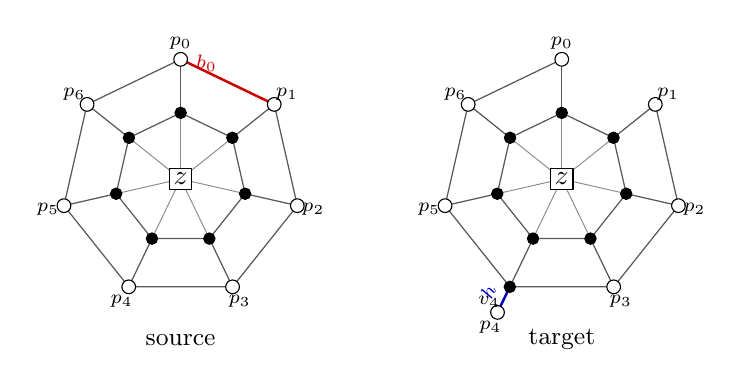
\begin{tikzpicture}[
    scale=.8,
    line join=round,
    edge/.style={draw=black!65, line width=.45pt},
    centeredge/.style={draw=black!45, line width=.35pt},
    internal/.style={circle, draw=black, fill=black, inner sep=1.45pt},
    port/.style={circle, draw=black, fill=white, inner sep=1.75pt, minimum size=4.5pt},
    centerport/.style={rectangle, draw=black, fill=white, inner sep=1.5pt, minimum size=6pt},
    labelstyle/.style={font=\scriptsize},
    bzero/.style={draw=red!80!black, line width=.9pt},
    hspike/.style={draw=blue!75!black, line width=.9pt}
  ]

    % ------------------------------------------------------------------
    % Source: seven observed outer ports, seven internal inner vertices,
    % and the observed centre z.
    % ------------------------------------------------------------------
    \begin{scope}
      \coordinate (sU0) at (90:1.05);
      \coordinate (sU1) at ({90-360/7}:1.05);
      \coordinate (sU2) at ({90-720/7}:1.05);
      \coordinate (sU3) at ({90-1080/7}:1.05);
      \coordinate (sU4) at ({90-1440/7}:1.05);
      \coordinate (sU5) at ({90-1800/7}:1.05);
      \coordinate (sU6) at ({90-2160/7}:1.05);
      \coordinate (sP0) at (90:1.9);
      \coordinate (sP1) at ({90-360/7}:1.9);
      \coordinate (sP2) at ({90-720/7}:1.9);
      \coordinate (sP3) at ({90-1080/7}:1.9);
      \coordinate (sP4) at ({90-1440/7}:1.9);
      \coordinate (sP5) at ({90-1800/7}:1.9);
      \coordinate (sP6) at ({90-2160/7}:1.9);
      \coordinate (sZ) at (0,0);

      % Centre spokes, inner cycle, radial edges, and outer cycle.
      \foreach \i in {0,...,6} {
        \draw[centeredge] (sZ) -- (sU\i);
      }
      \draw[edge] (sU0)--(sU1)--(sU2)--(sU3)--(sU4)--(sU5)--(sU6)--cycle;
      \draw[edge] (sU0)--(sP0);
      \draw[edge] (sU1)--(sP1);
      \draw[edge] (sU2)--(sP2);
      \draw[edge] (sU3)--(sP3);
      \draw[edge] (sU4)--(sP4);
      \draw[edge] (sU5)--(sP5);
      \draw[edge] (sU6)--(sP6);
      \draw[edge] (sP0)--(sP1)--(sP2)--(sP3)--(sP4)--(sP5)--(sP6)--cycle;
      \draw[bzero] (sP0) -- node[midway, above left, labelstyle, text=red!80!black] {$b_0$} (sP1);

      \node[internal] at (sU0) {};
      \node[internal] at (sU1) {};
      \node[internal] at (sU2) {};
      \node[internal] at (sU3) {};
      \node[internal] at (sU4) {};
      \node[internal] at (sU5) {};
      \node[internal] at (sU6) {};
      \node[port] at (sP0) {};
      \node[port] at (sP1) {};
      \node[port] at (sP2) {};
      \node[port] at (sP3) {};
      \node[port] at (sP4) {};
      \node[port] at (sP5) {};
      \node[port] at (sP6) {};
      \node[centerport] at (sZ) {$z$};
      \node[labelstyle] at (90:2.16) {$p_0$};
      \node[labelstyle] at ({90-360/7}:2.16) {$p_1$};
      \node[labelstyle] at ({90-720/7}:2.16) {$p_2$};
      \node[labelstyle] at ({90-1080/7}:2.16) {$p_3$};
      \node[labelstyle] at ({90-1440/7}:2.16) {$p_4$};
      \node[labelstyle] at ({90-1800/7}:2.16) {$p_5$};
      \node[labelstyle] at ({90-2160/7}:2.16) {$p_6$};
      \node[font=\small] at (0,-2.55) {source};
    \end{scope}

    % ------------------------------------------------------------------
    % Target: b_0 is absent.  The old outer p_4 is the internal vertex v_4;
    % the new observed p_4 is farther out and is attached by the blue spike.
    % ------------------------------------------------------------------
    \begin{scope}[xshift=6.05cm]
      \coordinate (tU0) at (90:1.05);
      \coordinate (tU1) at ({90-360/7}:1.05);
      \coordinate (tU2) at ({90-720/7}:1.05);
      \coordinate (tU3) at ({90-1080/7}:1.05);
      \coordinate (tU4) at ({90-1440/7}:1.05);
      \coordinate (tU5) at ({90-1800/7}:1.05);
      \coordinate (tU6) at ({90-2160/7}:1.05);
      \coordinate (tP0) at (90:1.9);
      \coordinate (tP1) at ({90-360/7}:1.9);
      \coordinate (tP2) at ({90-720/7}:1.9);
      \coordinate (tP3) at ({90-1080/7}:1.9);
      \coordinate (v4) at ({90-1440/7}:1.9);
      \coordinate (tP4) at ({90-1440/7}:2.35);
      \coordinate (tP5) at ({90-1800/7}:1.9);
      \coordinate (tP6) at ({90-2160/7}:1.9);
      \coordinate (tZ) at (0,0);

      \foreach \i in {0,...,6} {
        \draw[centeredge] (tZ) -- (tU\i);
      }
      \draw[edge] (tU0)--(tU1)--(tU2)--(tU3)--(tU4)--(tU5)--(tU6)--cycle;
      \draw[edge] (tU0)--(tP0);
      \draw[edge] (tU1)--(tP1);
      \draw[edge] (tU2)--(tP2);
      \draw[edge] (tU3)--(tP3);
      \draw[edge] (tU4)--(v4);
      \draw[edge] (tU5)--(tP5);
      \draw[edge] (tU6)--(tP6);

      % The outer cycle with b_0 removed, and the two old p_4 incidences
      % redirected to the internal v_4.
      \draw[edge] (tP1)--(tP2)--(tP3)--(v4)--(tP5)--(tP6)--(tP0);
      \draw[hspike] (v4) -- node[midway, sloped, above, labelstyle, text=blue!75!black] {$h$} (tP4);

      \node[port] at (tP0) {};
      \node[port] at (tP1) {};
      \node[port] at (tP2) {};
      \node[port] at (tP3) {};
      \node[port] at (tP4) {};
      \node[port] at (tP5) {};
      \node[port] at (tP6) {};
      \node[internal] at (tU0) {};
      \node[internal] at (tU1) {};
      \node[internal] at (tU2) {};
      \node[internal] at (tU3) {};
      \node[internal] at (tU4) {};
      \node[internal] at (tU5) {};
      \node[internal] at (tU6) {};
      \node[internal] at (v4) {};
      \node[labelstyle, below left] at (v4) {$v_4$};
      \node[centerport] at (tZ) {$z$};
      \node[labelstyle] at (90:2.16) {$p_0$};
      \node[labelstyle] at ({90-360/7}:2.16) {$p_1$};
      \node[labelstyle] at ({90-720/7}:2.16) {$p_2$};
      \node[labelstyle] at ({90-1080/7}:2.16) {$p_3$};
      \node[labelstyle] at ({90-1440/7}:2.61) {$p_4$};
      \node[labelstyle] at ({90-1800/7}:2.16) {$p_5$};
      \node[labelstyle] at ({90-2160/7}:2.16) {$p_6$};
      \node[font=\small] at (0,-2.55) {target};
    \end{scope}
  \end{tikzpicture}
  \caption{The full $n=7$ source and target before common boundary stripping.
    The move deletes the outer edge $b_0=p_0p_1$ and
    replaces the opposite outer vertex by an internal vertex $v_4$ with a
    new observed port $p_4$ attached by the spike $h$.  White vertices,
    including the boxed centre port $z$, are observed;
    black dots are internal vertices.}
  \label{fig:seven-move}
\end{figure}


\section{Determinantal construction of the uniform move}
\label{sec:operations}

A single circular minor $F_n$ vanishes on the common graph $H_n$
and is nonzero on either completion. Solving this vanishing condition
determines the selected feature; recovery on $H_n$ then determines
all inherited weights. We first record the boundary identities and
construct the missing connection.

Let \(Y\) be a finite loopless undirected graph with observed set \(B\), internal
set \(I\), and conductances \(c_e\).
Its Laplacian is
\[
 K_{uv}=-\sum_{e:u\leftrightarrow v}c_e\quad(u\ne v),\qquad
 K_{uu}=\sum_{e\ni u}c_e.
\]
Assume every connected component meets \(B\).
For strictly positive conductances the internal block is invertible, and
\begin{equation}
 \Lambda_Y=K_{BB}-K_{BI}K_{II}^{-1}K_{IB}.
 \label{eq:response}
\end{equation}
When \(I\) is empty, the determinant of the empty block is 1.
Over \(\QQ\), formula~\eqref{eq:response} defines a rational map into
\[
 \Vresp(B)=\{M=M^{\mathsf T}:M\one=0\},\qquad
 \dim\Vresp(B)=\binom{|B|}{2}.
\]
The entries $M_{uv}$ with $u<v$, for a fixed ordering of $B$,
are independent coordinates of this affine space.
The vertex \(z\) belongs to \(B\) throughout.

We use the following standard circular-planar results.
The graph \(\Pi_n\) is critical and has the standard medial matching
\cite[Corollary 1]{ABCC}. A critical graph remains critical after deletion
of a boundary edge or contraction of a boundary spike
\cite[Lemmas 11.1--11.2]{CIM}. Such a removal breaks some circular
connection. Criticality is equivalent both to recoverability and to
a lensless medial graph, and a critical medial matching determines
the connection set \cite[Section 7 and Lemmas 13.1--13.2]{CIM}.
Boundary conductance recovery with an observed center is
\cite[Lemma 10]{ABCC}. We record the formulas in our Laplacian convention.

\subsection{Exact boundary formulas}

For a boundary edge \(uv\), put
\[
 E_{uv}=(e_u-e_v)(e_u-e_v)^{\mathsf T},
\]
where \(e_u\) is the coordinate vector of the observed vertex.
Adding conductance \(q\) adds \(qE_{uv}\) to the response.

\begin{lemma}
\label{lem:spike}
If a spike of conductance \(h\) is inserted at observed vertex \(p\)
of a network with response \(N\), the response with the new observed
vertex bearing the same label is
\begin{equation}
 S_{p,h}(N)=N-\frac{N_{:,p}N_{p,:}}{h+N_{pp}}.
 \label{eq:spike-forward}
\end{equation}
The inverse operation is
\begin{equation}
 N=M+\frac{M_{:,p}M_{p,:}}{h-M_{pp}}.
 \label{eq:spike-inverse}
\end{equation}
Both are rational identities on their indicated domains.
For a positive spike, \(h-M_{pp}>0\).
\end{lemma}
\begin{proof}
The Schur pivot at the old observed vertex is \(h+N_{pp}\), giving
\eqref{eq:spike-forward}. Its \(p\)-column satisfies
\[
 M_{:,p}=\frac{h}{h+N_{pp}}N_{:,p},\qquad
 h-M_{pp}=\frac{h^2}{h+N_{pp}}>0.
\]
These identities give \eqref{eq:spike-inverse}.
\end{proof}

For any fixed square minor \(f\), define the polynomials
\[
 \Delta^f_{uv}(M)=f(M+E_{uv})-f(M),\qquad
 \beta^f_p(M)=f(M+M_{:,p}M_{p,:})-f(M).
\]
A determinant is affine in a rank-one update, so
\begin{align}
 f(M+sE_{uv})&=f(M)+s\Delta^f_{uv}(M),\label{eq:rank-edge}\\
 f(M+sM_{:,p}M_{p,:})&=f(M)+s\beta^f_p(M).
 \label{eq:rank-spike}
\end{align}
Each response update used here preserves symmetry and zero row sums,
since \(E_{uv}\one=0\) and \(M_{p,:}\one=0\).

\subsection{Circular connections and groves}

An ordered pair \(P=(a_1,\ldots,a_k)\), \(Q=(b_1,\ldots,b_k)\)
of disjoint outer observed vertices is circular if
\(a_1,\ldots,a_k,b_k,\ldots,b_1\) occurs in circular order in one
of the two orientations. A connection consists of vertex-disjoint
paths from \(a_j\) to \(b_j\), whose internal vertices are all internal
vertices of the network.

\begin{lemma}
\label{lem:grove}
Suppose deleting the central observed vertex \(z\) leaves a circular-planar
graph, with the given cyclic order of the other observed vertices.
For a circular pair \(P,Q\) avoiding \(z\),
\begin{equation}
 (-1)^k\det M_{P,Q}
 =\frac{Z_{P\mid Q}}{\det K_{II}},
 \label{eq:grove}
\end{equation}
where \(Z_{P\mid Q}\) is the sum of weights of spanning forests whose
boundary partition pairs \(a_j\) with \(b_j\) and leaves every other
observed vertex in its own boundary class.
For positive conductances this minor is nonzero, with sign \((-1)^k\),
exactly when the connection exists.
\end{lemma}
\begin{proof}
The all-minors matrix-tree theorem \cite{Chaiken} applies to
\[
 \det\begin{pmatrix}K_{II}&K_{IQ}\\K_{PI}&K_{PQ}\end{pmatrix}
 =\det K_{II}\,\det M_{P,Q}.
\]
Its omitted root sets are \(B\setminus P\) and \(B\setminus Q\).
Each component contains one root from each set. An unused observed
vertex belongs to both sets, so its component contains no other
observed vertex; this applies in particular to \(z\).
The pairing paths lie in the circular-planar graph with the unused
observed vertices deleted. Their unique noncrossing pairing gives
the sign \((-1)^k\) and \eqref{eq:grove}.
Conversely, a connection extends to a spanning forest with the required
partition by contracting its paths and the unused observed vertices
to roots and taking a rooted spanning forest. Every graph component
contains such a root. For positive conductances every forest weight
is positive, proving the stated equivalence.
\end{proof}

After boundary contractions, the same formula uses the current
observed vertices.

\subsection{The common missing connection}
\label{sec:connection}

Define \(F_n(M)=\det M_{P,Q}\) using Table~\ref{tab:minor}.
Integers in the table denote the labels \(p_i\).

\begin{table}[htbp]
\centering
\begin{tabular}{@{}ccll@{}}
\toprule
\(n\) & \(k\) & \(P\) & \(Q\)\\
\midrule
\(4L-1\) & \(2L-1\) & \((-j)_{j=0}^{2L-2}\) &
 \((1,\ldots,2L-1)\)\\
\(4L\) & \(2L-1\) & \((1,\ldots,2L-1)\) &
 \((-1,\ldots,-(2L-1))\)\\
\(4L+1\) & \(2L\) & \((1,\ldots,2L)\) &
 \((-1,\ldots,-2L)\)\\
\(4L+2\) & \(2L+1\) & \((0,-1,\ldots,-2L)\) &
 \((1,\ldots,2L+1)\)\\
\bottomrule
\end{tabular}
\caption{The common missing circular connection. All indices are modulo \(n\).}
\label{tab:minor}
\end{table}

\begin{proposition}
\label{prop:connection}
The connection in Table~\ref{tab:minor} is absent in \(H_n\) and present
in both \(X_n\) and \(X'_n\). Therefore, for every positive input,
\begin{equation}
 F_n(\Lambda_{H_n})=0,\qquad
 (-1)^kF_n(\Lambda_{X_n})>0,\qquad
 (-1)^kF_n(\Lambda_{X'_n})>0.
 \label{eq:connection-signs}
\end{equation}
\end{proposition}
\begin{proof}
Other observed vertices, including \(z\), cannot be used as transit
vertices. In \(H_n\), the following sets of \(k-1\) internal vertices
separate the relevant sides:
\begin{enumerate}
\item For \(n=4L-1\) or \(4L\), take columns \(0,2L\) on every
inner layer \(a=1,\ldots,L-1\).
For \(4L\), the corresponding outer vertices are unused observed
vertices. For \(4L-1\), the opposite outer vertex is unused and the
edge \(p_0p_1\) across the other cut is missing; \(p_0\), which is an
endpoint, stays on the \(P\)-side.
\item For \(n=4L+1\), take \(w_{0,2L}\) and columns \(0,2L\)
on the inner layers. The outer vertex in column 0 is the unused
observed vertex \(p_0\).
\item For \(n=4L+2\), take columns \(0,2L+1\) on all \(L\) layers.
The remaining external boundary edges join vertices on the same side;
the only source edge across the first cut has been deleted.
\end{enumerate}
Their sizes are \(2L-2,2L-1,2L\), respectively. After removing these
vertices and the unused observed vertices, no \(P\)-to-\(Q\) connection
can cross from one side to the other. Endpoints whose radial column
meets the separator also require a separator vertex. Thus \(k\)
disjoint paths cannot exist.

We now give the paths in the two completed graphs.
For \(4L-1\) and \(4L+2\), number a pair by \(j\), with endpoints
\(p_{-j},p_{j+1}\). For \(4L\) and \(4L+1\), use endpoints \(p_j,p_{-j}\).
A path assigned to a polygon layer follows its two endpoint columns
radially to that layer, traverses a polygon arc, and returns.
Call the arc through column 0 the first arc, and the other arc the
opposite arc.

Table~\ref{tab:paths} gives the layer assignments and the exceptional
pair indices. Both \(s\) and \(a\) denote actual polygon layer numbers:
the first three rows use only inner layers \(1,\ldots,L-1\), and the
last row includes the outer polygon layer \(0\).
The exceptional paths are:
\begin{itemize}
\item \(4L-1\): source pair \(j=0\) uses \(p_0p_1\);
target pair \(j=2L-2\) goes through the old \(p_{2L}\), now internal.
\item \(4L\): source pair \(j=1\) goes through the old \(p_0\);
target pair \(j=2L-1\) goes through the old \(p_{2L}\).
\item \(4L+1\): source pairs \(j=1,2L\) use the first and opposite
arcs of the outer polygon. Target pair \(j=2L\) uses the added external
edge, and pair \(j=2L-1\) uses the opposite outer polygon arc.
\item \(4L+2\): source pair \(j=0\) uses \(b_0\);
target pair \(j=2L\) uses the new external edge.
\end{itemize}

\begin{table}[htbp]
\centering
\begin{tabular}{@{}clll@{}}
\toprule
\(n\) & layer & source arc pair indices & target arc pair indices\\
\midrule
\(4L-1\) & \(s=1,\ldots,L-1\) &
 \(\substack{(s,\,2L-1-s)\\ \text{exception: }0}\) &
 \(\substack{(s-1,\,2L-2-s)\\ \text{exception: }2L-2}\)\\[4pt]
\(4L\) & \(s=1,\ldots,L-1\) &
 \(\substack{(s+1,\,2L-s)\\ \text{exception: }1}\) &
 \(\substack{(s,\,2L-1-s)\\ \text{exception: }2L-1}\)\\[4pt]
\(4L+1\) & \(s=1,\ldots,L-1\) &
 \(\substack{(s+1,\,2L-s)\\ \text{exceptions: }1,\,2L}\) &
 \(\substack{(s,\,2L-1-s)\\ \text{exceptions: }2L-1,\,2L}\)\\[4pt]
\(4L+2\) & \(a=0,\ldots,L-1\) &
 \(\substack{(a+1,\,2L-a)\\ \text{exception: }0}\) &
 \(\substack{(a,\,2L-1-a)\\ \text{exception: }2L}\)\\
\bottomrule
\end{tabular}
\caption{At each layer the first index uses the arc through column 0,
and the second uses the opposite arc. Exceptional pairs are assigned
once per graph by the paths in the text.}
\label{tab:paths}
\end{table}

For endpoints \((-j,j+1)\), the first arc has integer interval
\([-j,j+1]\) through 0, and the opposite arc has interval
\([j+1,n-j]\). For endpoints \((j,-j)\), these intervals are
\([-j,j]\) and \([j,n-j]\).
In each row of the table, the first index is strictly smaller than
the second; the two intervals at that layer are consequently disjoint.
As depth increases, the first index increases and the opposite index
decreases. Their deeper endpoint columns lie outside both arcs already
used on every shallower layer. The radial parts are therefore disjoint
from those arcs and from each other.

The exceptional outer paths listed above obey the same separation.
An external spike endpoint is distinct from the old polygon vertex;
thus a direct external edge does not occupy a vertex of a polygon
arc. Every pair is used exactly once, giving \(k\) vertex-disjoint
paths. Indeed, the source pair indices are \(0,\ldots,2L-2\),
\(1,\ldots,2L-1\), \(1,\ldots,2L\), and \(0,\ldots,2L\),
respectively. For each target, the exceptional pair or pairs are
the largest indices in the corresponding range, and the two
layer sequences partition all the remaining indices.
Empty inner-layer ranges for \(L=1\) cause no exception.
In particular, the first row of Table~\ref{tab:minor} then has \(P=(0)\).
Lemma~\ref{lem:grove} now gives \eqref{eq:connection-signs}.
\end{proof}

\subsection{Recovery on the common graph}
\label{sec:recovery}

Recover the common graph from the outside inward, stopping when all
innermost polygon vertices are observed.

\begin{lemma}
\label{lem:feature-recovery}
The boundary recovery formulas of \cite[Corollaries 4.3--4.4]{CIM}
and \cite[Lemma 10]{ABCC} are as follows.
Let a boundary edge or spike removal in the circular-planar graph
obtained by deleting \(z\) break a circular connection with minor \(f\).
For the complete response \(M\) including \(z\), its conductance is
\begin{align}
 c_{uv}&=\frac{f(M)}{\Delta^f_{uv}(M)}
 &&\text{for a boundary edge},\label{eq:recover-edge}\\
 c_p&=M_{pp}-\frac{\beta^f_p(M)}{f(M)}
 &&\text{for a boundary spike at \(p\)}.\label{eq:recover-spike}
\end{align}
For a spike the broken connection avoids \(p\).
On positive network inputs all indicated denominators are nonzero.
\end{lemma}
\begin{proof}
A connection with endpoint \(p\) survives contraction of its spike,
so a broken spike connection avoids \(p\).
By Lemma~\ref{lem:grove}, the minor is nonzero before removal and
zero afterwards. Substitute \(M-cE_{uv}\) for an edge and
\eqref{eq:spike-inverse} for a spike in the rank-one identities.
This gives \eqref{eq:recover-edge}--\eqref{eq:recover-spike}.
For a positive spike \(c-M_{pp}>0\); the identities then give
\(\Delta^f_{uv}=f/c\ne0\) or
\(\beta^f_p=-(c-M_{pp})f\ne0\), respectively.
\end{proof}

\begin{proposition}
\label{prop:base-recovery}
There is a finite rational map
\[
 \rec_n:\Vresp(B)\dashrightarrow\Aparam^{E(H_n)}
\]
with
\[
 \rec_n(\Lambda_{H_n}(c))=c
\]
for every strictly positive conductivity on \(H_n\).
It is regular at every \(\Lambda_{H_n}(b)\) with \(b>0\).
The same procedure works if the center star is omitted altogether.
\end{proposition}
\begin{proof}
For \(n=4L+2\), first recover and delete all remaining external
boundary edges. In all four cases, next recover and contract all remaining extra spikes,
so that every vertex of the outer polygon is observed.
If that polygon is not the innermost one, recover and delete its
remaining cycle edges. Every current outer observed vertex then has
degree one: its only incident edge is the next inward radial edge.
Recover and contract these radial spikes to expose the next layer.
Repeat until all innermost polygon vertices are observed.

The center star is incident to the innermost layer, so the outer
vertices being contracted retain degree one.
At termination all vertices, including \(z\), are observed.
The remaining innermost cycle edges, possibly with one edge missing,
and center edges are recovered as \(-M_{uv}\); their endpoints uniquely
determine the edge labels.

Deleting \(z\) initially gives a critical circular-planar graph:
it is \(\Pi_n\) after one legal boundary deletion or contraction.
Every subsequent step preserves criticality by the classical boundary
removal results. Thus each selected feature has a broken circular
connection. Enumerate circular pairs by size, ordered subset, and
cyclic cut; take the first witness. This finite choice depends only
on the graph, not on conductances. Apply
Lemma~\ref{lem:feature-recovery} at each step, retaining original edge
labels. This constructs \(\rec_n\) and recovers each conductance exactly.

All denominators are nonzero at every positive intermediate network.
Thus the composed recovery map is regular at every
\(\Lambda_{H_n}(b)\), \(b>0\).
Omitting the star changes only the last step:
the residual cycle is read directly, with no center edges.
\end{proof}

The response image of $H_n$ is Zariski-dense in the hypersurface $F_n=0$;
its algebraic description is given in
Corollary~\ref{cor:base-hypersurface} of Appendix~\ref{sec:effective}.

\subsection{Uniform reconstruction and the inverse transformation}
\label{sec:construction}

Here and below, \(\Delta,\beta\) without a superscript use the fixed
minor \(F_n\). For any specified completion of \(H_n\), define its
feature and stripped matrix by
\begin{align}
 \eta_{uv}(M)&=\frac{F_n(M)}{\Delta_{uv}(M)},&
 N_{uv}(M)&=M-\eta_{uv}(M)E_{uv},
 \label{eq:complete-edge}\\
 \eta_p(M)&=M_{pp}-\frac{\beta_p(M)}{F_n(M)},&
 N_p(M)&=M-\frac{F_n(M)}{\beta_p(M)}M_{:,p}M_{p,:}.
 \label{eq:complete-spike}
\end{align}
Both stripped matrices satisfy \(F_n(N)=0\).
The target edge endpoints or spike label are those in
Table~\ref{tab:features}. The source uses the edge \(p_0p_1\)
or the spike at \(p_0\).
The spike label is outside \(P\cup Q\) in every required case.

\subsubsection{Minor formulas for the opposite feature}

The boundary determinant ratios of \cite[Corollaries 4.3--4.4]{CIM}
take a particularly simple form for our fixed connection.
Write \(P^-,Q^-\) for \(P,Q\) with their last entries removed, and set
\[
 F_n^-(M)=\det M_{P^-,Q^-},\qquad
 C_{n,p}(M)=
 \det\begin{pmatrix}
 M_{P,Q}&M_{P,p}\\ M_{p,Q}&M_{pp}
 \end{pmatrix}.
\]
The index \(p\) in \(C_{n,p}\) is appended last in both lists.

\begin{proposition}
\label{prop:feature-minors}
For \(n=4L+1\) or \(4L+2\), the new edge conductance is
\begin{equation}
 q_t=-\frac{F_n(M)}{F_n^-(M)}.
 \label{eq:feature-edge-minor}
\end{equation}
For \(n=4L-1\) or \(4L\), the new spike at \(p=p_{2L}\) has conductance
\begin{equation}
 h_t=\frac{C_{n,p}(M)}{F_n(M)}.
 \label{eq:feature-spike-minor}
\end{equation}
In both formulas \(M=\Lambda_{X_n}(c)\). Their denominators are
nonzero and their values are strictly positive for every \(c>0\).
\end{proposition}
\begin{proof}
The target edge joins the last matched pair in
Table~\ref{tab:minor}. Adding \(qE_t\) changes only the last
diagonal entry of \(M_{P,Q}\), by \(-q\).
Hence \(\Delta_t(M)=-F_n^-(M)\), giving
\eqref{eq:feature-edge-minor}.
For a spike, expansion of the bordered determinant gives the
polynomial identity
\[
 C_{n,p}(M)=M_{pp}F_n(M)-\beta_p(M).
\]
Equation~\eqref{eq:complete-spike} gives
\eqref{eq:feature-spike-minor}.

For \(c>0\), the full connection exists by
Proposition~\ref{prop:connection}. Dropping its last path gives the
connection for \(P^-,Q^-\). Lemma~\ref{lem:grove} therefore gives
the signs \((-1)^k\) and \((-1)^{k-1}\) for \(F_n\) and \(F_n^-\),
respectively. Their negative ratio is strictly positive.

For the spike formula, temporarily count the outer vertex \(p\)
as internal, retaining every other observed vertex, including \(z\).
Write \(B'=B\setminus\{p\}\). The reduced response is
\[
 \widetilde M=
 M_{B',B'}
 -\frac{M_{B',p}M_{p,B'}}{M_{pp}},
 \qquad M_{pp}>0.
\]
Connectedness of \(X_n\) gives \(M_{pp}>0\), and the original
\(P\)-to-\(Q\) connection persists.
Lemma~\ref{lem:grove} gives
\((-1)^k\det\widetilde M_{P,Q}>0\), and the block determinant yields
\[
 C_{n,p}(M)=M_{pp}\det\widetilde M_{P,Q}.
\]
The numerator and denominator in
\eqref{eq:feature-spike-minor} thus have the same nonzero sign.
\end{proof}

The new feature is therefore positive for every positive source input.
The remaining positivity conditions will be expressed directly by the
center-edge minors in Section~\ref{sec:separation}.

\subsubsection{The complete transformation}

For \(Y=X_n\) or \(X'_n\), assemble \(\rec_n(N(M))\) and \(\eta(M)\)
in the edge order of \(Y\), and denote the resulting rational map by
\[
 \chart_Y:\Vresp(B)\dashrightarrow\Aparam^{E(Y)}.
\]

\begin{proposition}
\label{prop:charts}
For every positive network on either completion \(Y\),
\[
 \chart_Y(\Lambda_Y(c))=c.
\]
The maps \(\Lambda_Y\) and \(\chart_Y\) are birational inverses.
\end{proposition}
\begin{proof}
Removing the completion feature gives a positive actual
network on \(H_n\). Its minor is zero, whereas the completed
minor is nonzero by Proposition~\ref{prop:connection}.
Equations~\eqref{eq:complete-edge}--\eqref{eq:complete-spike},
derived exactly as in Lemma~\ref{lem:feature-recovery},
therefore recover the given feature and the stripped response.
Proposition~\ref{prop:base-recovery} then recovers all other conductances.
Every denominator is nonzero on the positive input.

This identity on an open real parameter set is a rational identity.
There are \(d\) parameters and \(d\) independent response coordinates.
Every parameter is a rational function of those response coordinates,
and each response coordinate is rational in the parameters. Thus
\[
 \QQ(c_e:e\in E(Y))
 =\QQ(\text{independent entries of }\Lambda_Y).
\]
The response coordinates are algebraically independent and generate
the function field. Hence \(\Lambda_Y\) is birational onto
\(\Vresp(B)\), with inverse \(\chart_Y\).

\end{proof}

In particular the transformation in Theorem~\ref{thm:main} is
\begin{equation}
 T_n=\chart_{X'_n}\circ\Lambda_{X_n},\qquad
 T_n^{-1}=\chart_{X_n}\circ\Lambda_{X'_n}.
 \label{eq:transformation}
\end{equation}
Proposition~\ref{prop:charts} proves the complete response identity and
the inverse identities. The formulas are uniform in \(n\): the graph
rules, the one minor, and the boundary-stripping order specify every
target edge conductance.

\section{Positive realization near the common degeneration}
\label{sec:positivity}

We now show that the rational transformation has a nonempty positive
domain near every positive common baseline. This supplies the initial
interval needed for the threshold theorem and the positive open set
used in proving locality.

\subsection{A transverse family at the common boundary}

Fix any positive conductivity \(b\) on \(H_n\), with response
\(M_0=\Lambda_{H_n}(b)\).
Use the degeneration ray $c_b(\varepsilon)$ of
\eqref{eq:positive-set}, and abbreviate its response as
$M(\varepsilon)=M_b(\varepsilon)$.
The source response is
\begin{align}
 M(\varepsilon)&=M_0+\varepsilon E_s
 &&\text{for an edge},\label{eq:source-edge-limit}\\
 M(\varepsilon)&=M_0-
 \frac{\varepsilon}{1+\varepsilon(M_0)_{00}}
 (M_0)_{:,0}(M_0)_{0,:}
 &&\text{for a spike}.\label{eq:source-spike-limit}
\end{align}
Thus it is rational and regular at \(\varepsilon=0\).

\begin{lemma}
\label{lem:positive-leading}
Write \(k=|P|\). The following numbers are nonzero:
\[
 \gamma_{\mathrm{src}}=
 \begin{cases}
 \Delta_s(M_0),&\text{source edge},\\
 -\beta_0(M_0),&\text{source spike}.
 \end{cases}
\]
They satisfy \((-1)^k\gamma_{\mathrm{src}}>0\), and
\begin{equation}
 F_n(M(\varepsilon))=
 \begin{cases}
 \gamma_{\mathrm{src}}\varepsilon,&\text{source edge},\\
 \gamma_{\mathrm{src}}\varepsilon/(1+\varepsilon(M_0)_{00}),
     &\text{source spike}.
 \end{cases}
 \label{eq:exact-family-minor}
\end{equation}
For a target edge \((-1)^k\Delta_t(M_0)>0\).
For a target spike \((-1)^{k+1}\beta_t(M_0)>0\).
\end{lemma}
\begin{proof}
Since \(F_n(M_0)=0\), the rank-one identities give the displayed formulas.
Adding any positive conductance on the source feature repairs the
connection in Proposition~\ref{prop:connection}.
For a source edge its minor is \(q\Delta_s(M_0)\).
For a source spike of conductance \(h\) it is
\[
 -\frac{\beta_0(M_0)}{h+(M_0)_{00}}.
\]
Lemma~\ref{lem:grove} gives the asserted nonzero signs.
Apply exactly the same argument to the target feature, whose addition
also repairs the connection.
\end{proof}

\subsection{Exact conductances along the degeneration}

The new feature has an exact rational formula along this family.
For either fixed minor \(A=F_n^-\) or \(A=C_{n,p}\), put
\[
 D_s^A=
 \begin{cases}
 \Delta_s^A(M_0),&\text{source edge},\\
 (M_0)_{00}A(M_0)-\beta_0^A(M_0),&\text{source spike}.
 \end{cases}
\]
The rank-one identities and \eqref{eq:exact-family-minor} give
\begin{align}
 q_t(\varepsilon)&=
 -\frac{\gamma_{\mathrm{src}}\varepsilon}
 {F_n^-(M_0)+\varepsilon D_s^{F_n^-}}
 &&(n=4L+1,\ 4L+2),\label{eq:exact-family-edge}\\
 h_t(\varepsilon)&=
 \frac{C_{n,p}(M_0)}{\gamma_{\mathrm{src}}\varepsilon}
 +\frac{D_s^{C_{n,p}}}{\gamma_{\mathrm{src}}}
 &&(n=4L-1,\ 4L).\label{eq:exact-family-spike}
\end{align}
For a source edge this follows by writing
\(A(M(\varepsilon))=A(M_0)+\varepsilon\Delta_s^A(M_0)\).
For a source spike the same calculation gives
\[
 A(M(\varepsilon))=
 \frac{A(M_0)+\varepsilon D_s^A}
 {1+\varepsilon(M_0)_{00}}.
\]
All coefficients are rational functions of the chosen baseline \(b\).
Proposition~\ref{prop:feature-minors} makes both feature formulas
positive for every \(\varepsilon>0\).

\begin{proposition}
\label{prop:positive-family}
For every $n\ge3$ and every positive $b$ on $H_n$,
the target conductances $T_n(c_b(\varepsilon))$ are strictly positive,
and all required denominators are nonzero, for sufficiently small \(\varepsilon>0\).
Every inherited target conductance tends to its value in \(b\).
On a compact subset of the positive baseline space, this convergence
and the choice of a sufficiently small positive \(\varepsilon\)
can be made uniform.
\end{proposition}
\begin{proof}
For a target edge, \eqref{eq:complete-edge} and
Lemma~\ref{lem:positive-leading} give
\[
 \eta_t(M(\varepsilon))
 =\frac{\gamma_{\mathrm{src}}}{\Delta_t(M_0)}\varepsilon+O(\varepsilon^2)>0 .
\]
The stripped matrix tends to \(M_0\).
For a target spike they give
\[
 \eta_t(M(\varepsilon))
 =\frac{-\beta_t(M_0)}{\gamma_{\mathrm{src}}}\varepsilon^{-1}+O(1)>0 .
\]
Here the coefficient of \(M_{:,t}M_{t,:}\) in the stripped matrix
is \(F_n(M(\varepsilon))/\beta_t(M(\varepsilon))=O(\varepsilon)\),
so the stripped matrix again tends to \(M_0\).

The map \(\rec_n\) is regular at \(M_0\) with value \(b\).
Its denominators therefore remain nonzero and all its output
conductances tend to their strictly positive baseline values.
The positive feature and these positive recovered conductances
give a positive actual target graph. Its internal Laplacian block
and the forward spike pivot are consequently nonzero.
Both sides of the rational right-inverse identity
\(\Lambda_{X'_n}\circ\chart_{X'_n}=\mathrm{id}\) are therefore
defined at \(M(\varepsilon)\), so this positive target has exactly
that response.
The source is positive for every finite \(\varepsilon>0\).

For uniformity, let \(b\) range over a compact positive set \(K\).
The normalized feature \(q_t/\varepsilon\) or
\(\varepsilon h_t\), and the stripped matrix, are rational functions
regular at every \((0,b)\), by the nonzero signs in
Lemma~\ref{lem:positive-leading}.
The same holds for the recovery expressions. The limiting scaled
feature and inherited conductances have positive minima on \(K\),
as do the absolute values of the nonvanishing divisors in these
regular expressions. Equation~\eqref{eq:exact-family-minor} controls
the remaining factor \(\varepsilon\) in \(F_n\).
A finite cover of \(K\) by neighborhoods where these inequalities
persist supplies one \(\varepsilon_0>0\) for the whole set.
\end{proof}

In the notation of \eqref{eq:positive-set},
Proposition~\ref{prop:positive-family} gives, for every $b>0$, a
$\delta(b)>0$ such that
\begin{equation}
 (0,\delta(b))\subset A_n(b).
 \label{eq:initial-interval}
\end{equation}
The local response geometry and an effective positive open box are
established in Appendix~\ref{sec:effective}.

\section{Locality and the common circular-planar cell}
\label{sec:locality}

The common circular-planar cell has two roles: it allows the same
exterior to be removed from both graphs, and it supplies the ordinary
response coordinates for the positivity criterion. We establish the
cell equality first, then recover the local move from its complete
interface response.

\subsection{The circular-planar target has the same medial matching}

Remove \(z\) and its incident edges to obtain the circular-planar
graphs \(C_n,C'_n\) and their common graph \(H_n^\circ\).

\begin{lemma}
\label{lem:target-critical}
The graph \(C'_n\) is critical and has the same medial matching as
\(C_n=\Pi_n\).
\end{lemma}
\begin{proof}
The star-free version of Proposition~\ref{prop:base-recovery}
recovers \(H_n^\circ\).
The paths and the missing connection in
Proposition~\ref{prop:connection} avoid \(z\), so they are unchanged.
For each positive network on \(C'_n\), the same single-minor
formulas recover its completion feature and its actual stripped
response, and then recover every conductance of \(H_n^\circ\).
Thus \(C'_n\) is recoverable for every positive conductivity.
By \cite[Lemma 13.2]{CIM} it is critical.

It has \(D=\binom n2\) edges.
The critical medial criterion excludes closed strands and
self-intersections and allows at most one intersection of each pair.
Thus its \(2n\) boundary endpoints belong to exactly \(n\) strands.
Each primal edge gives one intersection. Hence every pair of strands intersects once.
For any strand, each of the other \(n-1\) strands has one endpoint
on each side of its endpoints. In the cyclic order of the \(2n\)
medial boundary points, those endpoints are consequently \(n\)
positions apart. Its matching is
\(t_i\leftrightarrow t_{i+n}\).
This is the standard matching of \(\Pi_n\).
\end{proof}

By \cite[Theorems 2 and 4]{CIM}, $C_n$ and $C'_n$ therefore
have the same positive response cell, denoted $\cell_n$.
For either graph, the inverse response map on this cell is smooth
\cite[Theorem 4]{CIM}.

A boundary edge is \emph{exposed} if its exterior side faces the
intervening outer boundary arc in the star-free circular-planar graph.
The common-removal procedure uses exposed edges with two observed
endpoints and spikes of degree one at their observed endpoint in
the full graph, retaining the punctured-disk embedding.

In a critical circular-planar graph an edge between consecutive observed
vertices can be drawn exposed. Indeed, the region between it and the
empty boundary arc has no other observed vertex. A connection using
that region can only pair its two boundary endpoints, and can instead
use the edge itself. Any other edge in the region would therefore be
deletable without breaking a connection, contrary to criticality.
The region contains no such edges, and the edge may be moved to its
boundary arc.

\begin{lemma}
\label{lem:common-removal}
Suppose two critical circular-planar graphs have the same labelled
medial matching and a common exposed boundary edge at the same
position, or a common boundary spike at the same observed label.
After the same legal removal their labelled medial matchings and
connection sets remain equal.
\end{lemma}
\begin{proof}
Write \(t_{2i},t_{2i+1}\) for the medial endpoints just before and after
\(p_i\). A spike at \(p_i\) has a crossing directly adjacent to these
two endpoints. An exposed edge \(p_ip_{i+1}\) has a crossing directly
adjacent to \(t_{2i+1},t_{2i+2}\).
The common matching determines the other endpoints of the two strands.
The same deletion or contraction resolves the same four endpoints
in the same way; all other matched endpoints remain unchanged.
Boundary removal preserves criticality
\cite[Lemmas 11.1--11.2]{CIM}. The resulting matching determines the
connection set by the critical medial classification \cite[Section 7]{CIM}.
\end{proof}

\subsection{Common exterior conductances and the moving interface}

Starting with the two graphs, repeatedly remove common exposed boundary
edges and common genuine boundary spikes, checking legality in the
full graphs containing \(z\).
Here common means that the inherited edge label and both current
endpoint labels agree in the two graphs. In particular, a common
spike has the same observed label and the same internal neighbor.
At each iteration prefer edges, then spikes, and use the fixed edge-label
order. For definiteness label extra boundary edges, cycle edges,
radial edges, and extra spikes by their type, layer when present, and
cyclic index, and fix the corresponding lexicographic order.
Center edges are not candidates. The procedure stops when no
common legal feature remains. It is finite and depends only on the two
labelled embedded graphs. Let \(G_n,G'_n\) be the remaining graphs.

The circular-planar graphs at each stage remain critical and have
the same matching, by Lemmas~\ref{lem:target-critical} and
\ref{lem:common-removal}. Thus any circular connection broken on one
side by the selected removal is also broken on the other.
Lemma~\ref{lem:feature-recovery}, applied to the common complete
response including \(z\), recovers the same conductance on both sides.
Their updated complete responses also agree. This proves by induction,
on the positive domain of \(T_n\), that every removed exterior
conductance is unchanged and that
\begin{equation}
 \Lambda_{G_n}(c)=\Lambda_{G'_n}(d)
 \label{eq:core-equality}
\end{equation}
for the resulting core conductances. These identities are rational
identities, since they hold on a nonempty real open set.

Record each removed edge in a common exterior graph \(E_n^{\mathrm{ext}}\).
When a spike \(p_i v\) is removed, the old physical vertex \(p_i\)
remains in \(E_n^{\mathrm{ext}}\), and \(v\) becomes the new core interface vertex.
The \(i\)-th matrix slot keeps its logical index, but its physical
attachment is updated. Later radial removals update this interface
in the same way.
The center \(z\) remains observed throughout.

Reattaching \(E_n^{\mathrm{ext}}\) along the complete current interface reconstructs
the original source or target. For exterior conductances \(a\), let
\(\mathcal A_a(N)\) be this rational operation on a core response \(N\).
It is obtained by adjoining the exterior Laplacian and eliminating
the exterior internal vertices, or equivalently by reversing the
recorded boundary operations.
For positive core inputs it gives the complete original response.

\subsection{The local transformation is independent of the exterior}

Reattach the recorded exterior with all conductances equal to 1.
Composing this operation with the complete reconstruction gives a
left inverse for each core response map.

\begin{proposition}
\label{prop:local-independence}
There are rational maps
\[
 j_{G_n}=\pr_{G_n}\chart_{X_n}\mathcal A_{\one},\qquad
 j_{G'_n}=\pr_{G'_n}\chart_{X'_n}\mathcal A_{\one}
\]
that recover every positive core input from its complete
interface response. The core component of \(T_n(a,c)\) equals
\begin{equation}
 T_n^{\mathrm{loc}}(c)=j_{G'_n}(\Lambda_{G_n}(c)),
 \label{eq:local-map}
\end{equation}
as a rational identity, independently of \(a\).
This map is birational, with inverse
\(j_{G_n}\circ\Lambda_{G'_n}\).
\end{proposition}
\begin{proof}
Attach the fixed exterior \(E_n^{\mathrm{ext}}\) with all conductances equal to 1
to any positive target core.
The result is a positive network on \(X'_n\).
Its conductances are recovered by Proposition~\ref{prop:charts}.
Projecting to the core gives
\[
 j_{G'_n}(\Lambda_{G'_n}(d))=d.
\]
All divisions are defined on such a positive input.
The same argument applies to the source core.

On the positive domain of the complete transformation, common
exterior conductances are unchanged. Apply \(j_{G'_n}\) to
\eqref{eq:core-equality}; the target core is positive, so the identity
just proved gives \eqref{eq:local-map}.
Its right side contains no exterior parameter.
The positive domain is a nonempty Euclidean open set in all source
parameters, so this equality is also a rational identity.

The full positive domain contains a family point with exterior
parameters \(\one\), by Proposition~\ref{prop:positive-family}
with baseline \(b=\one\).
Choose a product neighborhood of this point inside the positive domain.
Its slice at exterior parameters \(\one\) is an open neighborhood
of the core parameters.
On this neighborhood the local formula is defined, the target
core is positive, and \eqref{eq:core-equality} holds.
Thus this response equality is a rational identity in the core parameters.
Applying the source local left inverse gives
\[
 (j_{G_n}\Lambda_{G'_n})\circ T_n^{\mathrm{loc}}=\mathrm{id}.
\]
The two core graphs have the same number of edges, since each common
step removes one edge on each side. A rational map between these
equal-dimensional affine parameter spaces with a rational left
inverse is birational, by the function-field argument of
Proposition~\ref{prop:charts}. The displayed map is its inverse.
\end{proof}

The selected source and target features remain in their respective cores.
Formula~\eqref{eq:local-map} gives a direct algorithm: attach the recorded
exterior with conductances 1 to the source core, compute its complete
response, apply the target reconstruction, and retain only target core
conductances.
The rational sample constructed in Appendix~\ref{sec:effective} has
exterior conductances \(\one\). Its core restriction and
Lemma~\ref{lem:polynomial-box} give a computable positive open box
for the local move.

\begin{corollary}
\label{cor:attachment}
Attach any common external network along the complete interface of
\(G_n,G'_n\). On the local positive applicability region, the response
on all remaining observed vertices is the same whenever the response
is defined. In particular an observed center port is preserved.
\end{corollary}
\begin{proof}
Eliminate the local internal vertices first.
The resulting matrices agree by \eqref{eq:core-equality}.
Adjoin the same exterior matrix and eliminate any remaining internal
vertices. Associativity of Schur complements gives equality of the
final complete responses.
\end{proof}

For \(n=3\) nothing is removed. For \(n=4\), remove the common
spike at \(p_1\). For \(n=5\), remove the common spikes at \(p_1,p_4\).
For \(n=6\), remove \(b_{-1},b_1\), then the common spikes at \(p_2,p_5\).
The remaining edge counts are respectively \(6,9,13,17\), giving the
small local patches of \cite{ABCC} after cyclic relabelling.
For \(n=7\), remove the four common outer edges
\(p_1p_2,p_2p_3,p_5p_6,p_6p_0\), then the radial spikes at
\(p_2,p_6\); the remaining
patch has 22 edges.
The common-removal procedure defines the local support for every \(n\).

Together, \eqref{eq:transformation},
Propositions~\ref{prop:feature-minors} and~\ref{prop:positive-family},
Lemma~\ref{lem:polynomial-box},
Proposition~\ref{prop:local-independence}, and
Corollary~\ref{cor:attachment} prove Theorem~\ref{thm:main}.

\section{Harmonic coordinates retaining the center}
\label{sec:harmonic}

The uniform move and its locality are now established. To determine
its full positive domain, we separate the ordinary response from the
currents at the center. We use the standard ground-state, or Doob,
conductance scaling
$c_{uv}\mapsto c_{uv}h_uh_v$; see
\cite[Proposition 2.1]{ACEM}. The boundary calculation below keeps
the center currents explicit and yields the realization coordinates.

Let $Y$ be either prescribed graph and let $C=Y-z$. Write
$V=V(C)$ and set
\[
 O=B\setminus\{z\}=\{p_0,\ldots,p_{n-1}\},\qquad
 I=V\setminus O.
\]
Let
$S=\{w_{L-1,0},\ldots,w_{L-1,n-1}\}$, with actual vertex
identifications understood. In particular, $S\cap O$ may be nonempty.
For a symmetric zero-row-sum matrix $M$ on $B$, put
\begin{equation}
 A=M_{O,O},\qquad j=A\one=-M_{O,z},\qquad
 \mathcal L=A-\diag(j).
 \label{eq:split}
\end{equation}
The pair $(\mathcal L,j)$ determines $M$: its center column is
$-j$ and its center diagonal is $\one^tj$.

\begin{lemma}
\label{lem:groundstate}
Suppose $M=\Lambda_Y(c)$ with $c>0$. Let $h$ be the harmonic
potential with $h_O=1$ and $h_z=0$. Then $h_v>0$ on $V$, and
the conductances
\[
 a_{uv}=c_{uv}h_uh_v\qquad(uv\in E(C))
\]
have ordinary circular-planar response $\Lambda_C(a)=\mathcal L$.
\end{lemma}
\begin{proof}
The maximum principle and the connectedness of $C$ give $h_v>0$.
Let $K$ be the Laplacian with the row and column of $z$ removed,
and put $D_h=\diag(h)$. The off-diagonal entries of $D_hKD_h$
are those of the Laplacian $K_a$ of $C$. Its internal row sums
vanish by harmonicity, and its outer row sums equal $j$.
Consequently
\begin{equation}
 D_hKD_h=K_a+\diag_O(j).
 \label{eq:groundstate-matrix}
\end{equation}
Taking the internal Schur complement, and using $h_O=1$, gives
$A=\Lambda_C(a)+\diag(j)$.
\end{proof}

For positive $a$ on $C$, let $G=K_a[I,I]^{-1}$. When $I$ is
empty, expressions involving this block are omitted. Define the
$O$-by-$S$ exit matrix
\begin{equation}
 \exitmat_C(a)_{:,s}=
 \begin{cases}
 e_s,&s\in S\cap O,\\
 (-K_a[O,I]G)_{:,s},&s\in S\cap I.
 \end{cases}
 \label{eq:exit-matrix}
\end{equation}
Its entries are nonnegative and its columns sum to one. The column
at an internal $s$ is the distribution of the unit current injected
there among the grounded outer ports.

\begin{proposition}
\label{prop:normal-form}
For either prescribed graph, positive conductances are in bijection
with pairs $(a,\mu)\in\RR_{>0}^{E(C)}\times\RR_{>0}^{S}$.
The map from these coordinates is
\begin{align}
 r_O&=\one,& r_I&=\one+G\mu_I,\label{eq:r-coordinate}\\
 c_{uv}&=a_{uv}r_ur_v,& c_{zs}&=r_s\mu_s.
 \label{eq:reconstruct}
\end{align}
Here $\mu$ is extended by zero off $S$. The corresponding full
response is given by
\begin{equation}
 A=\Lambda_C(a)+\diag(\exitmat_C(a)\mu).
 \label{eq:normal-response}
\end{equation}
For $a>0$ and $\mu\ge0$, the same formulas give a network with
strictly positive noncenter conductances and nonnegative center
conductances, still satisfying \eqref{eq:normal-response}.
Its zero center conductances are exactly the zero coordinates of $\mu$.
\end{proposition}
\begin{proof}
The inverse Dirichlet block $G$ is entrywise nonnegative, so
$r_I\ge1$. All conductances in \eqref{eq:reconstruct} are positive.
Set $j=\exitmat_C(a)\mu$. The internal equation in
\eqref{eq:r-coordinate} and the definition of $\exitmat_C$ give
\[
 K_ar=\mu-j^O,
\]
where $j^O\in\RR^V$ is the extension of $j$ by zero from $O$ to $V$.
Comparison of diagonal and
off-diagonal entries shows that the grounded Laplacian of
\eqref{eq:reconstruct} is
\[
 \diag(r)K_a\diag(r)+\diag_O(j).
\]
Its Schur complement is \eqref{eq:normal-response}.
This calculation also holds for $\mu\ge0$: then $r\ge1$, and
the grounded internal block is the positive definite matrix
$\diag(r_I)K_a[I,I]\diag(r_I)$.
Thus the response remains defined, including when every center
edge is absent, and $r_s\mu_s=0$ precisely when $\mu_s=0$.

Conversely, use $h$ from Lemma~\ref{lem:groundstate} and set
$r=1/h$, $a_{uv}=c_{uv}h_uh_v$, and $\mu_s=c_{zs}h_s$.
Equation~\eqref{eq:groundstate-matrix}, compared on the diagonal,
gives $K_ar=\mu-j^O$, hence \eqref{eq:r-coordinate}.
These operations are inverse to \eqref{eq:reconstruct}.
\end{proof}

\begin{lemma}
\label{lem:exit-invertible}
For $C=C'_n$ and every $a>0$, the matrix $\exitmat_C(a)$ is
invertible. More precisely, up to a fixed sign,
\begin{equation}
 \det K_a[V\setminus S,I]
 =\prod_{e\text{ radial or an outer spike}}a_e.
 \label{eq:cauchy-determinant}
\end{equation}
\end{lemma}
\begin{proof}
The all-minors matrix-tree theorem \cite{Chaiken} expresses the
determinant as a signed sum of forests having one root in $S$ and
one root in $O$ per component. Their root paths give $n$ disjoint
paths between the outer ports and the innermost polygon. Each
$n$-vertex layer is a separator, so these paths use every vertex of
that layer, one per path. A horizontal step would use two vertices
of a layer on one path and is impossible. The paths are therefore
exactly the radial columns and their outer spikes. They cover all
vertices, leaving no additional branches. An external edge joins
two outer roots and cannot occur. This is the unique contributing
forest, giving \eqref{eq:cauchy-determinant}. For $L=1$, coincident
outer and inner roots give zero-length paths; the same description
applies, with empty products allowed.

If $\exitmat_C(a)\mu=0$, set $u_O=0$ and $u_I=G\mu_I$.
Then $K_au=\mu$ on $V$, including its outer rows by
\eqref{eq:exit-matrix}. Thus
$K_a[V\setminus S,I]u_I=0$. Equation~\eqref{eq:cauchy-determinant}
implies $u=0$ and then $\mu=0$.
\end{proof}

\begin{corollary}
\label{cor:source-test}
Let $M$ be symmetric with zero row sums, and suppose its matrix
$\mathcal L$ from \eqref{eq:split} lies in $\cell_n$.
Recover the unique positive $a$ on $C'_n$ with response
$\mathcal L$, and put
\begin{equation}
 \mu=\exitmat_{C'_n}(a)^{-1}j.
 \label{eq:mu-test}
\end{equation}
Then $M$ has a positive realization on $X'_n$ if and only if
$\mu>0$. Such a realization is unique.
\end{corollary}
\begin{proof}
Necessity follows from the inverse in
Proposition~\ref{prop:normal-form} and uniqueness of the ordinary
recovery. For sufficiency, reconstruct by \eqref{eq:reconstruct}.
Its outer response block is $\mathcal L+\diag(j)=A$, and the
zero row sums recover the same center column and diagonal.
Lemma~\ref{lem:exit-invertible} and ordinary recovery also give
uniqueness.
\end{proof}

\section{A complete positivity test from response minors}
\label{sec:separation}

The preceding coordinates reduce positivity to $\mu_s>0$.
We now read each of these signs from a minor of the original full
response. The essential construction is a path family forced to use
one specified center edge, with a fixed endpoint pairing.

\subsection{Separating minors and center-source coordinates}

For disjoint ordered subsets $P,Q\subset B$ of cardinality $k$,
a full linkage means $k$ vertex-disjoint paths joining $P$ to $Q$,
with no other observed vertex in a path interior. For the Laplacian
sign convention used here, the all-minors forest identity is
\begin{equation}
 \det M_{P,Q}=(-1)^k
 \frac{\sum_\pi\operatorname{sgn}(\pi)Z_\pi}{Z_{\rm sep}}.
 \label{eq:forest-minor}
\end{equation}
The forest partition function $Z_\pi$ pairs each $P$ vertex with
its assigned $Q$ vertex and puts every other observed vertex in a
separate component. The denominator separates all observed vertices.
As in Lemma~\ref{lem:grove}, this is the all-minors matrix-tree
identity for the grounded Schur-complement minor, now with $z$
allowed among the paired endpoints.

\begin{definition}
A separating pair for a center edge $e_s$ is a pair $(P_s,Q_s)$
as above, with $z\in Q_s$, such that the target has a full linkage,
deleting $e_s$ destroys all full linkages, and every full linkage
has the same endpoint-permutation parity.
\end{definition}

\begin{lemma}
\label{lem:sign}
For a separating pair, let $\pi_s$ have its common parity and set
$\sigma_s=(-1)^k\operatorname{sgn}(\pi_s)$.
Then $f_s$ from \eqref{eq:separating-minor} is strictly positive on
every positive target response. It is zero on a target with $e_s$
deleted, all noncenter conductances positive, and the other center
conductances nonnegative.
\end{lemma}
\begin{proof}
All terms in the numerator of \eqref{eq:forest-minor} have the
same sign. A full linkage extends to a forest of the indicated
partition, so the numerator is nonzero for positive weights.
After deletion there is no full linkage, hence no such forest.
Further deletion of center edges cannot create a linkage. The
Dirichlet block remains invertible because the positive graph $C'_n$
is connected to the outer ports, even if $z$ is isolated.
\end{proof}

\begin{theorem}[Positive coordinates on the response fiber]
\label{thm:criterion}
For the separating pairs constructed in Lemma~\ref{lem:staircase},
over the cell $\cell_n$ there are strictly positive
functions $\kappa_s(\mathcal L)$ such that
\begin{equation}
 f_s(M)=\kappa_s(\mathcal L)\mu_s,
 \qquad \mu=\exitmat_{C'_n}(a)^{-1}j.
 \label{eq:minor-source}
\end{equation}
Consequently a symmetric zero-row-sum $M$ with
$\mathcal L\in\cell_n$ has a positive target realization exactly
when $f_s(M)>0$ for every $s$.
\end{theorem}
\begin{proof}
Fix $\mathcal L$, and hence the recovered $a$ and its invertible
exit matrix. Since $P_s$ and $Q_s$ are disjoint, the outer-to-outer
entries of the minor are off-diagonal entries of $\mathcal L$.
Its only column involving $j$ is the center column $-j$.
Thus $f_s$ is homogeneous linear in $j$, and hence in $\mu$.

Take $\mu_s=0$ and all other $\mu$ coordinates positive.
Formulas~\eqref{eq:r-coordinate}--\eqref{eq:reconstruct} still
construct a network with all noncenter conductances positive and
exactly the center edge $e_s$ deleted. Lemma~\ref{lem:sign} gives
$f_s=0$. A linear function vanishing on this relatively open part
of the coordinate hyperplane must be a scalar multiple of $\mu_s$.
Taking all $\mu$ coordinates positive shows that this scalar is
strictly positive. Corollary~\ref{cor:source-test} now proves the
claimed equivalence.
\end{proof}

Thus the required positive response region, over a fixed
$\mathcal L$, is the simplicial cone
$\exitmat_{C'_n}(a)\RR_{>0}^{S}$ in the variable $j$.
The minors are positively rescaled coordinates of this cone.
We next construct the separating pairs for every prescribed graph.

\subsection{Uniform staircase separators}
\label{sec:staircase}

\subsubsection{Endpoint sets}

Let $D$ be the target's set of outer spike indices and let $E$
index its external edges $p_ip_{i+1}$. Directly from
Table~\ref{tab:features}, these data are as in
Table~\ref{tab:target-boundary}. The vertices $w_{j,i}$ retain
their labels after any boundary identification.

\begin{table}[htbp]
\centering
\begin{tabular}{@{}lll@{}}
\toprule
$n$ & $D$ & Other target boundary data\\
\midrule
$4L-1$ & $\{2L\}$ & missing polygon edge $w_{0,0}w_{0,1}$\\
$4L$ & $\{1,\ldots,2L\}$ & none\\
$4L+1$ & $(\mathbb Z/n)\setminus\{0\}$ & $E=\{2L\}$\\
$4L+2$ & $\mathbb Z/n$ &
$E=\{-L,\ldots,-1\}\cup\{1,\ldots,L\}\cup\{2L+1\}$\\
\bottomrule
\end{tabular}
\caption{Boundary data for the prescribed targets.}
\label{tab:target-boundary}
\end{table}

Fix $s$ and write
\[
 a=s-L,\qquad b=s+L,\qquad
 \delta_a=\mathbf1_{a\in D},\quad \delta_b=\mathbf1_{b\in D}.
\]
In this section $a,b$ are indices, not conductance vectors.
Intervals below follow increasing cyclic order, with the length
specified by the displayed integer endpoints. Choose the consecutive
outer block
\begin{equation}
 P_s=\{s-L+1,\ldots,s+L-1\}
       \cup(\{a,b\}\cap D),
 \qquad k=2L-1+\delta_a+\delta_b.
 \label{eq:P-set}
\end{equation}
Initially take the outer part of $Q_s$ to be all remaining indices,
except $a$ and $b$ when they have no spike. Make the corrections
in Table~\ref{tab:corrections}, and then include $z$ in $Q_s$.
Finally order both sets by $p_0,\ldots,p_{n-1},z$ for computing
the determinant and its permutation sign.

\begin{table}[htbp]
\centering
\small
\begin{tabular}{@{}p{.12\linewidth}p{.31\linewidth}p{.49\linewidth}@{}}
\toprule
$n$ & Condition & Correction to the outer part of $Q_s$\\
\midrule
$4L-1$ & $a=2L$ or $b=2L$ &
Add back the other, nonspiked endpoint among $a,b$.\\[3pt]
$4L$ & all $s$ & No correction.\\[3pt]
$4L+1$ & $a=0$ & Delete $2L+1$.\\
       & $b=0$ & Delete $2L$.\\[3pt]
$4L+2$ & $a-1\in E$ & Delete $a-1$.\\
       & $b\in E$ & Delete $b+1$.\\
\bottomrule
\end{tabular}
\caption{The boundary corrections in the staircase construction.
Unlisted cases require no correction.}
\label{tab:corrections}
\end{table}

The sets are disjoint and have equal cardinality $k$. For $n=4L$,
exactly one of $a,b$ lies in the consecutive half-circle $D$.
For $n=4L+2$, the sets $E$ and $E+(2L+1)$ are complementary,
so exactly one of the last two corrections applies. For $n=4L-1$,
the exceptional centers are $s=L,3L$; for $n=4L+1$, they are
$s=L,3L+1$. Counting the added or omitted endpoints verifies
the equality in each case. The outer part of $Q_s$ is a consecutive
block separated from $P_s$.

\subsubsection{The separator and the path family}

Define
\begin{equation}
\begin{split}
 T_s={}&\{w_{j,s-(L-j)},w_{j,s+(L-j)}:1\le j<L\}\\
 &\cup\{w_{0,a}:a\in D\}\cup\{w_{0,b}:b\in D\}.
\end{split}
\label{eq:staircase-cut}
\end{equation}
The displayed vertices are distinct and $|T_s|=k-1$.
Between the two staircases, row $j$ has the indices
\begin{equation}
 s-(L-j)+1,\ldots,s+(L-j)-1.
 \label{eq:wedge-interior}
\end{equation}
The last row contains only $w_{L-1,s}$.

\begin{figure}[htbp]
\centering
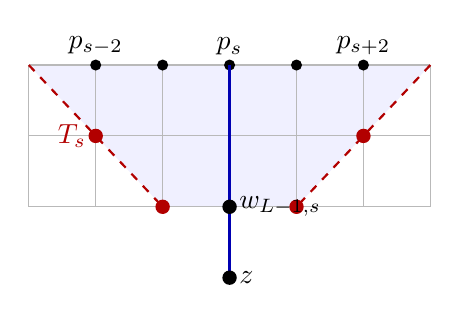
\begin{tikzpicture}[x=.85cm,y=.9cm]
 \fill[blue!6] (-3,0)--(3,0)--(1,-2)--(-1,-2)--cycle;
 \foreach \j in {0,1,2} {
   \foreach \i in {-3,-2,-1,0,1,2} {
     \draw[gray!55] (\i,-\j)--({\i+1},-\j);
   }
 }
 \foreach \j in {0,1} {
   \foreach \i in {-3,-2,-1,0,1,2,3} {
     \draw[gray!55] (\i,-\j)--(\i,{-\j-1});
   }
 }
 \draw[red!70!black,dashed,thick] (-3,0)--(-2,-1)--(-1,-2);
 \draw[red!70!black,dashed,thick] (3,0)--(2,-1)--(1,-2);
 \foreach \x/\y in {-2/-1,-1/-2,2/-1,1/-2} {
   \fill[red!70!black] (\x,\y) circle (2.6pt);
 }
 \foreach \i in {-2,-1,0,1,2} {
   \fill (\i,0) circle (2pt);
 }
 \draw[blue!70!black,very thick] (0,0)--(0,-3);
 \fill (0,-2) circle (2.6pt);
 \fill (0,-3) circle (2.6pt) node[right] {$z$};
 \node[above] at (0,0) {$p_s$};
 \node[right] at (0,-2) {$w_{L-1,s}$};
 \node[above] at (-2,0) {$p_{s-2}$};
 \node[above] at (2,0) {$p_{s+2}$};
 \node[left,red!70!black] at (-2,-1) {$T_s$};
\end{tikzpicture}
\caption{The staircase geometry for $L=3$. The full polygon grid
is unwrapped into rows to locate the separator, and only the central
center edge is drawn. The actual boundary edges, spikes, and port
identifications are specified in Tables~\ref{tab:target-boundary}
and~\ref{tab:corrections}.}
\label{fig:staircase}
\end{figure}

\begin{lemma}
\label{lem:staircase}
For every $n\ge3$ and every center index $s$, the sets
\eqref{eq:P-set} and Table~\ref{tab:corrections} form a separating
pair for $e_s$. In fact the endpoint pairing is unique, and pairs
$p_s$ with $z$.
\end{lemma}
\begin{proof}
We prove separation, existence, and uniqueness in turn.

\emph{Separation.}
Remove the unselected observed vertices, which cannot occur on a
linkage. Each horizontal or radial edge leaving
\eqref{eq:wedge-interior} meets $T_s$, except possibly at the two
outer endpoints $a,b$. The boundary rules handle these exceptions
as follows. For $4L-1$, ordinarily both endpoints are unselected.
At an exceptional center one is a spike endpoint in $T_s$; the
other is in $Q_s$, but its only polygon edge into the wedge is
the missing edge $0$--$1$. When $L\ge2$, its inward radial
edge also lies outside the wedge; when $L=1$, there is no
interlayer radial edge.
For $4L$, the nonspiked endpoint is unselected and the spiked
one is blocked by $T_s$.

For $4L+1$, the added external edge can cross the wedge boundary
only when $a=0$ or $b=0$. The corresponding correction removes
its exterior observed endpoint. For $4L+2$, the complementary
half-circle property of $E$ leaves exactly one external edge
crossing the two sides; its exterior observed endpoint is again
removed. Other external edges join observed points on the same
side and do not bypass the separator.

The only innermost vertex inside the wedge is $w_{L-1,s}$.
Deleting $T_s$ and $e_s$ therefore separates $P_s$ from $Q_s$.
Since $|T_s|=k-1$, there is no full linkage after deleting $e_s$.

\emph{Existence.}
Join $p_s$ to $z$ by its radial column, including its outer spike
if present and then $e_s$. Put
$r_+=L-1+\delta_b$ and $r_-=L-1+\delta_a$.
List $Q_s\setminus\{z\}$ as $q_1,\ldots,q_{k-1}$ in increasing
cyclic order, starting immediately after the rightmost endpoint
$p_{s+r_+}$ of the $P_s$ block and skipping unselected ports.
The explicit pairing is
\begin{equation}
 p_s\longleftrightarrow z,\qquad
 p_{s+r}\longleftrightarrow q_{r_+-r+1}\ (1\le r\le r_+),
 \qquad
 p_{s-r}\longleftrightarrow q_{r_++r}\ (1\le r\le r_-).
 \label{eq:explicit-pairing}
\end{equation}
Since $r_++r_-=k-1$, these assignments use all endpoints once.
On each side the outermost $P_s$ endpoint is paired with the
nearest $Q_s$ endpoint.

For $p_{s\pm r}$, descend along its column to layer $L-r$,
follow that polygon in increasing cyclic index order for $p_{s+r}$
and decreasing cyclic index order for $p_{s-r}$ until reaching its
assigned $Q_s$ column, and ascend to the observed endpoint. Include outer
spikes at the ends where necessary. On each side, nested endpoint
intervals have strictly increasing depths. A deeper horizontal
segment lies below the radial ends of a shallower path, while its
own radial ends lie outside the shallower horizontal interval.
Thus the paths are disjoint on that side. The left and right
intervals are disjoint and both avoid the central column.

A depth-zero path occurs only at a spiked endpoint $a$ or $b$.
Normally it uses one polygon edge. When an adjacent $Q_s$ endpoint
was omitted in the $4L+1$ or $4L+2$ case, it uses two; the
intermediate vertex is the internal end of an unused spike, not
an observed vertex. In the $4L-1$ exceptional cases, the
depth-zero path starts at $2L$ and does not use the missing
$0$--$1$ edge. All other horizontal segments are internal.
This constructs a full linkage.

\emph{Uniqueness of pairing.}
Add $w_{L-1,s}$ to $T_s$, obtaining a separator of size $k$.
Any full linkage must use every separator vertex and exactly one
per path.

First let $L=1$, so $n\in\{3,4,5,6\}$, and put $v=w_{0,s}$.
The two neighboring polygon indices are $a=s-1$ and $b=s+1$.
Each spiked neighbor belongs to $T_s$. For $n=4,5$, each
nonspiked neighbor is an unselected observed vertex; for $n=6$
both neighbors are spiked. For $n=3$, a nonspiked neighbor is
either unselected or is the exceptional endpoint added back to
$Q_s$; in the latter case its edge to $v$ is the missing
$0$--$1$ edge. Thus every polygon exit from $v$ is blocked by
$T_s$, an unselected observed vertex, or a missing edge.
If $s\in D$, the only remaining directions at $v$ are its spike
to $p_s$ and its center edge to $z$. Since a linkage path cannot
use a second separator vertex, the path through $v$ is
$p_s,v,z$. If $s\notin D$, then $v=p_s$, and the same restriction
forces its path to be the edge $p_sz$; other observed vertices
cannot be path interiors, and no external edge is incident to
such an unspiked $p_s$ in these four targets.
The remaining outer endpoints have
the unique reverse-order pairing by planar disjointness.
This proves the claim for $L=1$.

Now let $L\ge2$. A path through $w_{L-1,s}$ must end at $z$:
its radial neighbor is inside the wedge and both
innermost polygon neighbors belong to $T_s$. Reaching any other
outside endpoint would require a second separator vertex.
All separator vertices are internal. Work in the embedded graph
after deleting the unselected observed vertices and their incident
edges. Consecutive vertices on either staircase are opposite corners
of an interlayer quadrilateral. Join them by an arc whose interior
lies in that open face. At the bottom, join $w_{L-1,s-1}$ to
$w_{L-1,s}$ and then to $w_{L-1,s+1}$ by arcs in the two adjacent
faces toward layer $L-2$, with their interiors off the innermost
polygon edges. The left and right arcs have disjoint interiors:
their face interiors are disjoint, and the two bottom arcs meet
only at $w_{L-1,s}$.

Extend the two outer ends to the disk boundary on the respective
sides of the $P_s$ block. The missing edge, deleted unselected
endpoints, and external-edge corrections checked in the separation
step provide the required gaps in the remaining graph. Choose the
extensions through these gaps, keeping any corner spikes with
endpoints in $P_s$ on the $P_s$ side. The resulting simple arc meets
the remaining graph exactly at $T_s\cup\{w_{L-1,s}\}$, in the
order down the left staircase, through the bottom vertex, and up
the right staircase. Together with the outer boundary arc containing
$P_s$, it bounds a disk.

Truncate each linkage path at its first separator vertex. These
disjoint segments lie in that disk and end at all $k$ separator
vertices. Two segments with alternating endpoints on the disk
boundary would intersect, so the matching to the separator is
forced by boundary order. Its exits are the left staircase, the
bottom vertex, and the right staircase. There are
$L-1+\delta_a$ exits to the left of the bottom vertex and
$L-1+\delta_b$ to its right, exactly the numbers of $P_s$
endpoints on the two sides of $p_s$. Hence the path ending at
$z$ starts at $p_s$ in this case as well. The remaining endpoints lie in two separated
outer arcs, for which planar disjointness forces the unique
reverse-order pairing. This proves uniqueness and therefore the
required common permutation parity; the pairing is
\eqref{eq:explicit-pairing}.
\end{proof}

\begin{proof}[Proof of Theorem~\ref{thm:source-positivity}]
For a positive source, Lemma~\ref{lem:groundstate} places
$\mathcal L$ in the positive response cell of $C_n$, which equals
$\cell_n$ by Lemma~\ref{lem:target-critical} and the circular-planar
response-cell theorem. Lemma~\ref{lem:staircase} constructs the
separating pairs. Theorem~\ref{thm:criterion} gives the stated
criterion, and Corollary~\ref{cor:source-test} gives uniqueness.
\end{proof}

\section{Non-reentry and the positivity threshold}
\label{sec:ray}

The full-response criterion turns the ray problem into simultaneous
sign conditions. The rank-one response formulas make these conditions
affine after multiplication by a common positive denominator.

\begin{lemma}
\label{lem:rank-one}
Let $M_0=\Lambda_{H_n}(b)$. For the two source feature types,
\begin{equation}
 M_b(\varepsilon)=
 \begin{cases}
 M_0+\varepsilon vv^t,&v=e_0-e_1,\quad\text{source edge},\\[2pt]
 M_0-\dfrac{\varepsilon}{1+m\varepsilon}uu^t,
       &u=(M_0)_{:,0},\ m=(M_0)_{00},\quad\text{source spike}.
 \end{cases}
 \label{eq:rank-one}
\end{equation}
Here $m>0$. Every fixed response minor is affine in
$\varepsilon$ in the edge case, and has an affine numerator
over $1+m\varepsilon$ in the spike case.
\end{lemma}
\begin{proof}
The response formulas are \eqref{eq:source-edge-limit} and
\eqref{eq:source-spike-limit}; connectedness gives $m>0$.
Column multilinearity makes every minor affine in the rank-one
update parameter. Substituting $-\varepsilon/(1+m\varepsilon)$
gives the asserted affine numerator in the spike case.
\end{proof}

\begin{proof}[Proof of Theorem~\ref{thm:nonreentry}]
The source is positive for every $\varepsilon>0$, so
Theorem~\ref{thm:source-positivity} gives \eqref{eq:ray-criterion}.
Lemma~\ref{lem:rank-one} gives its affine numerators and common
positive denominator.

By \eqref{eq:initial-interval}, each numerator
$\alpha_s+\beta_s\varepsilon$ is positive for sufficiently
small positive $\varepsilon$. Thus $\alpha_s\ge0$, and
$\alpha_s=0$ requires $\beta_s>0$. If $\beta_s<0$, its
positivity set is precisely
$(0,\alpha_s/(-\beta_s))$; otherwise it is the whole positive
axis. Intersecting these conditions proves the interval assertion
and \eqref{eq:threshold}.

Suppose the threshold is finite. The source remains strictly
positive at $\varepsilon_*$. Its $\mathcal L$ is still in
$\cell_n$, so the ordinary recovered conductances $a$ have
finite positive values there. Ordinary recovery and the
invertibility in Lemma~\ref{lem:exit-invertible} make $a$ and
$\mu$ continuous at this point. Approaching from the positive
interval gives $\mu\ge0$ in the limit, with at least one zero
coordinate; otherwise positivity would continue past the threshold.
Equations~\eqref{eq:r-coordinate}--\eqref{eq:reconstruct} now give
$r_I\ge1$, finite strictly positive $a_{uv}r_ur_v$, and finite
nonnegative $r_s\mu_s$. Their zero coordinates are exactly the
vanishing center edges, as claimed.
\end{proof}

For a concrete computation of \eqref{eq:threshold}, let
$\alpha_s=f_s(M_0)$. In the edge case,
$\beta_s=f_s(M_b(1))-\alpha_s$. In the spike case,
\[
 \beta_s=(1+m)f_s(M_b(1))-\alpha_s.
\]
These two evaluations of the original full response determine all
coefficients in the threshold formula.

\subsection{An exact seven-sided threshold}
\label{sec:checks}

Consider the $n=7$ edge family, with source edge $p_0p_1$ of
conductance $\varepsilon$. Specify its common baseline by
Table~\ref{tab:baseline}; every displayed entry is divided by $100$.
The separating minors give
\[
 \varepsilon_* = \frac{54997063108}{61616096925}.
\]
\begin{table}[htbp]
\centering
\begin{tabular}{@{}lll@{}}
\toprule
Inherited edges & Index order & $100$ times the conductances\\
\midrule
$w_{0,i}w_{0,i+1}$ & $i=1,\ldots,6$ & $103,110,117,105,112,100$\\
$w_{1,i}w_{1,i+1}$ & $i=0,\ldots,6$ & $107,114,102,109,116,104,111$\\
$w_{0,i}w_{1,i}$ & $i=0,\ldots,6$ & $118,106,113,101,108,115,103$\\
$zw_{1,i}$ & $i=0,\ldots,6$ & $110,117,105,112,100,107,114$\\
\bottomrule
\end{tabular}
\caption{The positive baseline for the seven-sided example.}
\label{tab:baseline}
\end{table}
The active minor is the one for $e_2$, with
\[
 P_2=(1,2,3,4),\qquad Q_2=(0,5,6,z),\qquad \sigma_2=-1.
\]
For this baseline its affine coefficients are
\[
 \alpha_2=\frac{791977108969211347}{6438130505517017250000},
 \qquad
 \beta_2=-\frac{47322321642570149}{343366960294240920000}.
\]
All other selected minors have nonnegative slope in this example.
At this threshold the center edge $e_2$ vanishes, while all
noncenter conductances stay strictly positive. An exact recovery over
$\mathbb Q(\varepsilon)$ gives the same value and verifies equality
of the full $8\times8$ response matrices; the computational records
are listed in Appendix~\ref{sec:computations}.

\appendix

\section{The finite algorithm}
\label{sec:algorithm}

The input is an integer \(n\ge3\) and a strictly positive source
conductance vector \(c\). First decide positive target realizability
by \eqref{eq:full-source-criterion}; on the positive domain, recover
the unique target weights and record the divisors used.

\paragraph{Precomputation for \(n\).}
Construct the three labelled graphs in Table~\ref{tab:features}
and the ordered pair in Table~\ref{tab:minor}. Fix the
boundary-stripping sequence of Proposition~\ref{prop:base-recovery}.
At each step, enumerate circular connections in the star-free graph
in a fixed order and retain the first one broken by that step.
Existence of a witness follows from criticality. Existence of each
connection is a finite graph problem: enumerate simple paths and
test their allowed internal vertices and required disjointness.
These graph and witness data are reused for every input on \(X_n\).
Also construct the center-edge pairs of Section~\ref{sec:staircase}
and their signs from \eqref{eq:explicit-pairing}.

\paragraph{Evaluation at \(c\).}
Compute the complete response and test the separating minors before
performing target recovery.
\begin{enumerate}
\item Compute the complete source response \(M=\Lambda_{X_n}(c)\)
using the internal set specified by the source graph.
If any $f_s(M)\le0$, return \emph{no strictly positive target}.
Otherwise continue with the following recovery steps, recording each
divisor. All these divisors are nonzero by Proposition~\ref{prop:charts},
applied to the positive target supplied by the criterion.
\item Evaluate the appropriate formula in
\eqref{eq:complete-edge} or \eqref{eq:complete-spike} at the
target position in Table~\ref{tab:features}. Retain the new
conductance \(\eta\) and the stripped response \(N\).
\item Apply the precomputed stripping sequence to \(N\), using
\eqref{eq:recover-edge}--\eqref{eq:recover-spike} and the exact
response updates. Read the final innermost cycle and center
conductances from the remaining off-diagonal entries.
\item Assign these values to the inherited target edge labels and
assign \(\eta\) to the new feature, obtaining \(c'\).
\end{enumerate}
Return the positive vector \(c'\) and the recorded divisors.
The inverse rational map is evaluated by computing the target response
and using the source completion formulas on their domain of definition,
as in Proposition~\ref{prop:charts}.
For a fixed degeneration ray, the two response evaluations in
Section~\ref{sec:ray}, following its main proof, determine
$\alpha_s,\beta_s$ and hence the threshold \eqref{eq:threshold}.

\section{Local response geometry and effective applicability}
\label{sec:effective}

\subsection{The common response hypersurface}

\begin{corollary}
\label{cor:base-hypersurface}
The Zariski closure of the response image of \(H_n\) is
\[
 \mathcal H_n=\{M\in\Vresp(B):F_n(M)=0\}.
\]
This is an irreducible hypersurface of dimension \(d-1\).
On a nonempty open subset of it,
\(\Lambda_{H_n}(\rec_n(M))=M\).
\end{corollary}
\begin{proof}
The row and column sets of \(F_n\) are disjoint, so its \(k^2\)
entries are distinct independent coordinates in \(\Vresp(B)\).
The determinant of a generic matrix is irreducible: the singular
matrix locus is the closure of the image of products of
\(k\)-by-\((k-1)\) and \((k-1)\)-by-\(k\) matrices, and the determinant
has multiplicity one at a rank-\((k-1)\) point.
For \(k=1\) it is simply a coordinate.

The parameter space of \(H_n\) is irreducible. Its rational left
inverse in Proposition~\ref{prop:base-recovery} makes the image
closure have dimension \(|E(H_n)|=d-1\).
Proposition~\ref{prop:connection} places that closure in
\(\mathcal H_n\). Equal dimensions and irreducibility give equality,
and the two inverse identities follow on their common rational domain.
\end{proof}

\subsection{The common positive response neighborhood}

\begin{corollary}
\label{cor:positive-boundary}
Let \(\Omega_Y=\Lambda_Y(\RR_{>0}^{E(Y)})\) denote the positive
response image. Every \(M_0=\Lambda_{H_n}(b_0)\), \(b_0>0\),
has a neighborhood \(W\) in \(\Vresp(B)\) such that
\[
 \Omega_{X_n}\cap W
 =\Omega_{X'_n}\cap W
 =\{M\in W:(-1)^kF_n(M)>0\}.
\]
In particular,
\[
 \Lambda_{H_n}(\RR_{>0}^{E(H_n)})
 \subset
 \partial\bigl(\Omega_{X_n}\cap\Omega_{X'_n}\bigr).
\]
\end{corollary}
\begin{proof}
The identity \(\rec_n\circ\Lambda_{H_n}=\mathrm{id}\), with
\(\rec_n\) regular at \(M_0\), shows that
\(D\Lambda_{H_n}\) has rank \(d-1\) at \(b_0\).
Its image lies in \(\ker dF_n\).

For either completion \(Y\), let \(\Phi_Y(s,b)\) be its response
with feature conductance \(s\) for an edge or \(s^{-1}\) for a spike.
The boundary formulas extend this map smoothly to \(s=0\), where
\(\Phi_Y(0,b)=\Lambda_{H_n}(b)\).
Lemma~\ref{lem:positive-leading}, applied to the feature of \(Y\),
gives
\[
 (-1)^k\frac{\partial}{\partial s}
 F_n(\Phi_Y(s,b_0))\bigg|_{s=0}>0.
\]
Thus \(dF_n\ne0\) at \(M_0\), and the \(s\)-direction is transverse
to the \(d-1\) baseline directions. The inverse function theorem
makes \(\Phi_Y\) a local chart onto a neighborhood \(W_Y\) of \(M_0\).
Shrink its parameter neighborhood so that \(b>0\).
The exact boundary formulas show that
\((-1)^kF_n(\Phi_Y(s,b))\) has the sign of \(s\) there.
Consequently every matrix on the positive side in \(W_Y\) is the
response of a positive completion.
Conversely, every positive completion lies on this side by
Proposition~\ref{prop:connection}.
Take \(W=W_{X_n}\cap W_{X'_n}\). The asserted equality follows,
and \(F_n(M_0)=0\) places each positive common response on its boundary.
\end{proof}

\subsection{Computable applicability conditions}

The finite algorithm tests applicability by rational inequalities.
We now construct a positive rational input and an open box on which
all these inequalities hold.

\begin{lemma}
\label{lem:polynomial-box}
Given finitely many rational functions defined at a rational point
\(c_*\), whose required nonzero values and required signs are known,
one can compute a rational open box about \(c_*\) preserving them.
\end{lemma}
\begin{proof}
List the finitely many polynomial numerators and denominators of all
required divisions, signs, and determinants; orient each nonzero
polynomial so that its value at \(c_*\) is positive.
Expand
\[
 p(c_*+u)=p(c_*)+\sum_{\alpha\ne0}p_\alpha u^\alpha,\qquad
 A_p=\sum_{\alpha\ne0}|p_\alpha|.
\]
Set \(r_p=1\) if \(A_p=0\), and otherwise
\[
 r_p=\min\left(1,\frac{p(c_*)}{2A_p}\right).
\]
For \(\|u\|_\infty<r_p\le1\), the nonconstant part has absolute value
less than \(p(c_*)/2\). Take the minimum of these bounds and, when
positive input coordinates are required,
\(\frac12\min_e(c_*)_e\).
This is a positive rational radius.
\end{proof}

To obtain \(c_*\) effectively, take \(b=\one\) and substitute the
family \(c_{\one}(\varepsilon)\)
into the finite formulas. Normalize the feature as
\(\eta_t/\varepsilon\) for a target edge or
\(\varepsilon\eta_t\) for a target spike.
The normalized feature and all other target conductances have positive
limits at 0. For every required polynomial factor remove its power of
\(\varepsilon\) and orient its nonzero constant term positively.
The factors controlling recovery divisions have nonzero limits by
Proposition~\ref{prop:base-recovery}.
For each resulting polynomial
\(p(\varepsilon)=p_0+\sum_{j\ge1}p_j\varepsilon^j\), \(p_0>0\), take
\[
 \delta_p=
 \begin{cases}
 1,&\sum_{j\ge1}|p_j|=0,\\
 \min(1,p_0/(2\sum_{j\ge1}|p_j|)),&\text{otherwise}.
 \end{cases}
\]
Their finite minimum \(\delta_n\) is positive and rational.
Choose \(\varepsilon_{\rm test}=\delta_n/2\).
Then \(c_*=c_{\one}(\varepsilon_{\rm test})\) is a rational positive input with positive
output and all divisions defined.
Lemma~\ref{lem:polynomial-box} gives the box \(U_n\).
In particular, $0<\varepsilon_{\rm test}<\varepsilon_*(\one)$.

\section{A three-sided formula and its positive domain}
\label{sec:three-example}

The three-sided move was obtained in \cite[Appendix A]{ABCC}.
It illustrates the uniform construction in our labels.
For \(n=3\), all four source vertices \(p_0,p_1,p_2,z\) are observed.
Write
\[
 a=c_{p_0p_1},\quad b=c_{p_2p_0},\quad d=c_{p_1p_2},
 \qquad u=c_{zp_0},\quad v=c_{zp_1},\quad w=c_{zp_2},
 \qquad s=b+d+w.
\]
The target removes \(p_0p_1\), makes the old \(p_2\) an internal
vertex \(v_2\), and attaches the new observed \(p_2\) by a spike
of conductance \(h\). The target conductances are
\begin{align*}
 h&=s+\frac{bd}{a},&
 \widehat b&=b+\frac{as}{d},&
 \widehat d&=d+\frac{as}{b},\\
 \widehat u&=u-\frac{aw}{d},&
 \widehat v&=v-\frac{aw}{b},&
 \widehat w&=w\left(1+\frac{as}{bd}\right).
\end{align*}
The edges carrying \(\widehat b,\widehat d,\widehat w\) meet \(v_2\).

Indeed, \(F_3(M)=M_{01}=-a\),
\(\beta_2(M)=M_{02}M_{21}=bd\), and \(M_{22}=s\).
Equations~\eqref{eq:complete-spike} give
\[
 h=s+\frac{bd}{a},\qquad
 N=M+\frac{a}{bd}M_{:,2}M_{2,:}.
\]
The entry \(N_{01}\) is zero; the other five off-diagonal entries
and the zero row sums give the common graph's Laplacian.
Inserting the spike using Lemma~\ref{lem:spike} recovers \(M\).

For strictly positive source conductances, all six target conductances
are strictly positive if and only if
\[
 0<a<\min\left(\frac{ud}{w},\,\frac{vb}{w}\right).
\]
Every displayed divisor and the spike pivot are then nonzero.
This is the three-sided instance of the threshold in
Theorem~\ref{thm:nonreentry}.

\section{Exact computational records}
\label{sec:computations}

Table~\ref{tab:computations} summarizes the exact checks accompanying
the constructions. Response calculations use rational arithmetic.
The programs, their local dependencies, and the recorded certificates
are collected in the
\href{supplementary/punctured_disk_moves_and_rays_supplement.zip}
{combined computational archive}. Its README gives the directory
layout and complete running commands, and its SHA-256 manifest fixes
the supplied files. Both the move and ray modules are included.

\begin{table}[htbp]
\centering
\small
\begin{tabular}{@{}p{.55\linewidth}p{.37\linewidth}@{}}
\toprule
Calculation & Recorded range\\
\midrule
Missing-connection paths and separators & $n=3,\ldots,30$\\
Missing minors and feature formulas & $n=3,\ldots,14$\\
Complete transformation, inverse and locality & $n=3,\ldots,10$\\
Center-edge staircase paths and deletion cuts & $n=3,\ldots,40$; $817$ cases\\
Separating minors and linkage calculations & $n=3,\ldots,16$\\
Signed center-coordinate matrix & $n=3,\ldots,10$\\
Full symbolic ray response and exact threshold & $n=7$\\
\bottomrule
\end{tabular}
\caption{Finite exact checks for the uniform constructions.}
\label{tab:computations}
\end{table}

The staircase entry program is
\nolinkurl{verify_wedge_structure.py};
\nolinkurl{verify_wedge_witnesses.py} checks the minors and their
affine formulas at a third parameter after fitting two values.
The program \nolinkurl{audit_minor_coordinates.py} constructs the
responses for $\mu=e_t$ independently and verifies that the matrix
$f_s(M_{e_t})$ is diagonal with positive diagonal entries. Its signs
are fixed by the explicit pairing in \eqref{eq:explicit-pairing}.
The seven-sided threshold and baseline coefficients are recorded in
\nolinkurl{wedge_witness_certificate.json}, and agree with the
independent $\mathbb Q(\varepsilon)$ recovery certificate.

\section*{Acknowledgments}

This mathematical paper was prepared with the assistance of artificial intelligence.  I
first acknowledge the textual data produced by humanity as a whole, which
provides the linguistic and cultural record from which mathematical expression
can be learned.  I then thank the accumulated scholarly achievements of
mathematicians throughout history.  I also thank the researchers whose work has
advanced and refined neural networks through successive generations.  Finally,
I thank the OpenAI team for the training and development of the models used in
the preparation of this paper.

\begin{thebibliography}{9}
\bibitem{ABCC}
Y. Alexandr, B. Burks, S. Chepuri, and P. Commins,
\emph{Recovering conductances of resistor networks in a punctured disk},
arXiv:1812.01517v1, 2018.
\url{https://arxiv.org/abs/1812.01517v1}.

\bibitem{Chaiken}
S. Chaiken,
A combinatorial proof of the all minors matrix tree theorem,
\emph{SIAM Journal on Algebraic Discrete Methods} \textbf{3} (1982),
no.~3, 319--329.
\url{https://doi.org/10.1137/0603033}.

\bibitem{CIM}
E. B. Curtis, D. Ingerman, and J. A. Morrow,
Circular planar graphs and resistor networks,
\emph{Linear Algebra and its Applications} \textbf{283} (1998), 115--150.
\url{https://doi.org/10.1016/S0024-3795(98)10087-3}.

\bibitem{KW}
R. Kenyon and D. B. Wilson,
\emph{The space of circular planar electrical networks},
arXiv:1411.7425.
\url{https://arxiv.org/abs/1411.7425}.

\bibitem{ALT}
J. Alman, C. Lian, and B. Tran,
\emph{Circular Planar Electrical Networks II: Positivity Phenomena},
arXiv:1309.3011v1.
\url{https://arxiv.org/abs/1309.3011v1}.

\bibitem{ACEM}
C. Ara\'uz, \'A. Carmona, A. M. Encinas, and M. Mitjana,
Green functions on product networks,
\emph{Discrete Applied Mathematics} \textbf{263} (2019), 22--34.
\url{https://doi.org/10.1016/j.dam.2018.10.004}.
\end{thebibliography}

\end{document}
